\chapter{More on Coordinate Bases, Linear Transformations}
\label{chap:6x}

In this chapter, we will go deeper into what a matrix actually represents in the big picture. Matrices, by nature, are the rules of \textit{linear transformations} (or \textit{linear mappings}) between two vector spaces. We are going to study several special types of linear transformations, and this ultimately reveals the relationship between any $n$-dimensional real vector space and the real $n$-space $\mathbb{R}^n$, as an \textit{isomorphism}. We will then move to discuss how a change of coordinates works for vectors and matrices, as well as the \textit{Gram-Schmidt} process to make an \textit{orthonormal} basis. This is needed in Earth Science as we often have to switch between different coordinate systems/bases (e.g.\ wind shear/motion-relative coordinates for tropical cyclones) and particularly want to work with the nicer ones that facilitate computation.

\section{Ideas of Linear Transformations}
\label{section:lineartrans}

\subsection{Linear Transformations between Vector Spaces}

Consider two vector spaces, we may want to know if vectors in one of the vector spaces, let's say $\mathcal{U}$, can be associated to or \textit{transformed} into vectors in another vector space $\mathcal{V}$, according to some rules. This is known as a \index{Transformation}\index{Mapping}\keywordhl{transformation/mapping} from the vector space $\mathcal{U}$ to $\mathcal{V}$. Of the most concern is the class of \index{Linear Transformation/Mapping}\keywordhl{linear transformations/mappings} which obeys the two properties listed below.
\begin{defn}[Linear Transformation/Map]
\label{defn:lintrans}
A linear transformation (also called a linear map) from a vector space $\mathcal{U}$ to another vector space $\mathcal{V}$ is a mapping: $T: \mathcal{U} \to \mathcal{V}$, such that for all possible pairs of vectors $\vec{u}^{(1)}, \vec{u}^{(2)} \in \mathcal{U}$, and any scalar $a$, it satisfies:
\begin{enumerate}
    \item $T(\vec{u}^{(1)} + \vec{u}^{(2)}) = T(\vec{u}^{(1)}) + T(\vec{u}^{(2)})$ (Additivity), and
    \item $T(a\vec{u}^{(j)}) = aT(\vec{u}^{(j)})$ (Homogeneity).
\end{enumerate}
These two properties combined are known as \index{Linearity}\keywordhl{linearity}. An equivalent condition is then $T(a\vec{u}^{(1)} + b\vec{u}^{(2)}) = aT(\vec{u}^{(1)}) + bT(\vec{u}^{(2)})$, where $b$ is any scalar as well.
\end{defn}
Notice that if $\mathcal{U}$/$\mathcal{V}$ coincides with the real $n$/$m$-space $\mathbb{R}^n$/$\mathbb{R}^m$, and we express any vector $\vec{u} \equiv [\vec{u}]_\beta$\footnote{We use "$\equiv$" to associate any vector to its representation in some fixed coordinate system.} in $\mathcal{U}$ by $n$ coordinates using some basis $\mathcal{\beta}$ (similarly for $\vec{v} \equiv [\vec{v}]_{\eta} \in \mathcal{V}$ that has $m$ coordinates in some basis $\mathcal{\eta}$), then $\smash{[T]_\beta^{\eta}} = A$, where $A$ is any $m \times n$ matrix, will satisfy the requirements of and is a linear transformation from $\mathcal{U}$ to $\mathcal{V}$ according to the rule $T(\vec{u}) \equiv \smash{[T]_\beta^{\eta}}[\vec{u}]_\beta = A[\vec{u}]_\beta$. (Short Exercise: show this satisfies the conditions outlined in Definition \ref{defn:lintrans} above!\footnotemark) This implies that all matrices can be considered as some sort of linear mappings (for now, between $\mathbb{R}^n$ and $\mathbb{R}^m$). In fact, the converse, which states that any linear transformation (between finite-dimensional vector spaces) can be represented by a matrix, is also true as well, and will be discussed in the following parts of this section. \par
Provided that $\mathcal{U}$/$\mathcal{V}$ is $n$/$m$(finite)-dimensional, let's now explicitly fix a basis $\mathcal{\beta} = \{\vec{u}^{(1)}, \vec{u}^{(2)}, \ldots, \vec{u}^{(n)}\}$ for $\mathcal{U}$ (again, similarly we have $\mathcal{\eta} = \{\vec{v}^{(1)}, \vec{v}^{(2)}, \ldots, \allowbreak \vec{v}^{(m)}\}$ for $\mathcal{V}$). For each $\vec{u}^{(j)}$, $j = 1,2,\ldots,n$, denote $\vec{w}^{(j)} = T(\vec{u}^{(j)})$ as the resulting vectors in $\mathcal{V}$ after applying the transformation $T$ over the basis vectors for $\mathcal{U}$. Notice that $[\vec{u}^{(j)}]_\beta = (e^{(j)})_\beta$ where the $j$-th basis vector of $\mathcal{\beta}$ is explicitly represented in the coordinate form with the $j$-th entry being $1$ and others being $0$ (where the usual hat symbol on $e$ is not present) relative to the $\mathcal{\beta}$ system. Due to Definition \ref{defn:coordRn} and Properties \ref{proper:lincombofspan}, $T(\vec{u}^{(j)}) = \vec{w}^{(j)} \in \mathcal{V}$ can be expressed as a \textit{unique} linear combination as $\vec{w}^{(j)} = \smash{a_1^{(j)}}\vec{v}^{(1)} + \smash{a_2^{(j)}}\vec{v}^{(2)} + \cdots + \smash{a_m^{(j)}}\vec{v}^{(m)} = \sum_{i=1}^{m} \smash{a_i^{(j)}}\vec{v}^{(i)}$ of the basis vectors $\vec{v}^{(i)}$ from $\mathcal{\eta}$, i.e.\ \footnotetext{$T(\vec{u}^{(1)}+\vec{u}^{(2)}) \equiv A([\vec{u}^{(1)}]_\beta + [\vec{u}^{(2)}]_\beta) = A[\vec{u}^{(1)}]_\beta + A[\vec{u}^{(2)}]_\beta \equiv T(\vec{u}^{(1)})+T(\vec{u}^{(2)})$ and $T(a\vec{u}^{(1)}) \equiv A(a[\vec{u}^{(1)}]_\beta) = a(A[\vec{u}^{(1)}]_\beta) \equiv aT(\vec{u}^{(1)})$}
\begin{align}
T(\vec{u}^{(j)}) = \sum_{i=1}^{m} a_i^{(j)}\vec{v}^{(i)}
\end{align}
The matrix formed by the above coefficients $A = \smash{a_i^{(j)}}$ is then the desired, \textit{unique} \index{Matrix Representation of a Linear Transformation}\keywordhl{matrix representation} of our linear transformation $T$. To see this, insert $\vec{u}^{(j)}$ and compare both sides of $T(\vec{u}) \equiv A[\vec{u}]_\beta$. Subsequently,
\begin{align*}
A[\vec{u}^{(j)}]_\beta &= a_i^{(j)}(e^{(j)})_\beta \\
&=
\begin{bmatrix}
a_1^{(1)} & a_1^{(2)} & \cdots & a_1^{(j)} & \cdots & a_1^{(n)} \\
a_2^{(1)} & a_2^{(2)} & & a_2^{(j)} & & a_2^{(n)} \\
\vdots & & & \vdots & & \vdots \\
a_m^{(1)} & a_m^{(2)} & \cdots & a_m^{(j)} & \cdots & a_m^{(n)}
\end{bmatrix}
\begin{bmatrix}
0 \\
0 \\
\vdots \\
1 {\scriptsize \text{ (the $j$-th entry)}} \\
\vdots \\
0 {\scriptsize \text{ (the last index is $n$)}}
\end{bmatrix} \\
&=
\begin{bmatrix}
a_1^{(j)} \\
a_2^{(j)} \\
\vdots \\
a_m^{(j)}
\end{bmatrix}
\end{align*}
Due to the structure of $(e^{(j)})_\beta$, this matrix product yields exactly the $j$-th column of $A = \smash{a_i^{(j)}}$ as shown above (see the remark under Properties \ref{proper:linearcombmatrix}). Moreover, the coordinates of $\vec{w}^{(j)} = T(\vec{u}^{(j)})$ in the $\mathcal{\eta}$ system
\begin{align*}
T(\vec{u}^{(j)}) \equiv [T(\vec{u}^{(j)})]_\eta &= [\vec{w}^{(j)}]_\eta \\
&= [\sum_{i=1}^{m} a_i^{(j)}\vec{v}^{(i)}]_\eta \\
&= \sum_{i=1}^{m} a_i^{(j)}[\vec{v}^{(i)}]_\eta \\
&= \sum_{i=1}^{m} a_i^{(j)}(e^{(i)})_\eta \\
&=  a_1^{(j)} \begin{bmatrix}
1 \\
0 \\
\vdots \\
0
\end{bmatrix}
+
a_2^{(j)} \begin{bmatrix}
0 \\
1 \\
\vdots \\
0
\end{bmatrix}
+ \cdots
+
a_m^{(j)} \begin{bmatrix}
0 \\
0 \\
\vdots \\
1 {\scriptsize \text{ (the last index is $m$)}}
\end{bmatrix}
\\
&= \begin{bmatrix}
a_1^{(j)} \\
0 \\
\vdots \\
0
\end{bmatrix}
+
\begin{bmatrix}
0 \\
a_2^{(j)} \\
\vdots \\
0
\end{bmatrix}
+ \cdots
+
\begin{bmatrix}
0 \\
0 \\
\vdots \\
a_m^{(j)}
\end{bmatrix}
=
\begin{bmatrix}
a_1^{(j)} \\
a_2^{(j)} \\
\vdots \\
a_m^{(j)}
\end{bmatrix}
\end{align*}
also gives the same $j$-th column of $A_{ij} = \smash{a_i^{(j)}}$. By the same argument, this holds for any $j$. Hence, the association of the matrix $\smash{[A]_\beta^\eta} = \smash{a_i^{(j)}}$ to the linear transformation $T$ is consistent, where we have now added the subscript $\beta$ and superscript $\eta$ to emphasize the transformation is carried out in reference to these two specific coordinate bases. This same line of reasoning also shows that, to construct the matrix representation of a linear transformation, we compute $T(\vec{u}^{(j)}) = \vec{w}^{(j)}$ for each of the $\vec{u}^{(j)}$ in the $\mathcal{\beta}$ basis and find its coordinates in the $\mathcal{\eta}$ frame, namely $[\vec{w}^{(j)}]_\eta$, which readily become the $j$-th column of the matrix to be found. To be more clear, we have
\begin{align}
[T]_\beta^\eta &= 
\begin{bmatrix}
[T(\vec{u}^{(1)})]_\eta | [T(\vec{u}^{(2)})]_\eta | \cdots | [T(\vec{u}^{(n)})]_\eta
\end{bmatrix} \nonumber \\
&=
\begin{bmatrix}
[\vec{w}^{(1)}]_\eta | [\vec{w}^{(2)}]_\eta | \cdots | [\vec{w}^{(n)}]_\eta
\end{bmatrix} \nonumber \\
&= 
\begin{bmatrix}
a_1^{(1)} & a_1^{(2)} & \cdots & a_1^{(n)} \\
a_2^{(1)} & a_2^{(2)} &  & a_2^{(n)} \\
\vdots & & \ddots & \vdots \\
a_m^{(1)} & a_m^{(2)} & \cdots & a_m^{(n)}
\end{bmatrix}
= a_i^{(j)} = [A]_\beta^\eta
\end{align}
Notice that here the $i$/$j$ subscript/superscript has been exchanged when compared to like Properties \ref{proper:linsysmat}.
\begin{defn}[Matrix Representation of a Linear Transformation]
\label{defn:matrixrepoflintrans}
A linear transformation $T: \mathcal{U} \to \mathcal{V}$ as defined in Definition \ref{defn:lintrans} between two finite-dimensional vector spaces, with respect to the bases $\mathcal{\beta} = \{\vec{u}^{(1)}, \vec{u}^{(2)}, \ldots, \vec{u}^{(n)}\}$ for $\mathcal{U}$ and $\mathcal{\eta} = \{\vec{v}^{(1)}, \vec{v}^{(2)}, \ldots, \vec{v}^{(m)}\}$ for $\mathcal{V}$, has a unique matrix representation of
\begin{align*}
[T]_\beta^\eta = 
\begin{bmatrix}
a_1^{(1)} & a_1^{(2)} & \cdots & a_1^{(n)} \\
a_2^{(1)} & a_2^{(2)} &  & a_2^{(n)} \\
\vdots & & \ddots & \vdots \\
a_m^{(1)} & a_m^{(2)} & \cdots & a_m^{(n)}
\end{bmatrix}
\end{align*}
where the entries $\smash{a_i^{(j)}}$ are those found according to the relations $T(\vec{u}^{(j)}) = \sum_{i=1}^{m} \smash{a_i^{(j)}}\vec{v}^{(i)}$, or in matrix notation, $\smash{[T]_\beta^\eta} [\vec{u}]_\beta = [\vec{v}]_\eta$.
\end{defn}
\begin{proper}
\label{proper:sametrans}
For two linear transformations $S$ and $T$, if $S(\vec{v}) = T(\vec{v})$ for all $\vec{v} \in \mathcal{V}$, then $S = T$ must be the same linear transformation.
\end{proper}
Let's illustrate how it works out using an easy example using the familiar $\mathbb{R}^n$ and $\mathbb{R}^m$. 
\begin{exmp}
\label{exmp:lineartransmatrixrep}
Let $\mathcal{U} = \mathbb{R}^3$ and $\mathcal{V} = \mathbb{R}^2$, it can be easily verified that $\mathcal{\beta} = \{(1,2,1)^T, (0,1,-1)^T, (2,-1,1)^T\}$ is a basis for $\mathcal{U}$, and the same goes for $\mathcal{V}$ with a basis $\mathcal{\eta} = \{(1,2)^T, (2,-1)^T\}$. If a linear transformation $T: \mathbb{R}^3 \to \mathbb{R}^2$ obeys the rule $T((x,y,z)^T) = (x+2y, x-y+z)^T$ (by the way, you should verify if this is really a linear transformation), find its matrix representation $\smash{[T]_\beta^\eta}$ with respect to the $\mathcal{\beta}$ and $\mathcal{\eta}$ system. Then, use the results to compute $T((-1,4,-1)^T)$.
\end{exmp}
\begin{solution}
Following Definition \ref{defn:matrixrepoflintrans}, we set out to find how the linear transformation will be applied on the basis vectors in $\mathcal{\beta}$. For the first one, we have
\begin{align*}
T((1,2,1)^T) = ((1)+2(2), (1)-(2)+(1))^T = (5,0)^T
\end{align*}
which can be subsequently written as a linear combination of the two basis vectors in $\mathcal{\eta}$:
\begin{align*}
(5,0)^T = 1(1,2)^T + 2(2,-1)^T
\end{align*}
Hence $a_1^{(1)} = 1$, $a_2^{(1)} = 2$, and this gives us the first column of $[T]_\beta^\eta$ as
\begin{align*}
\begin{bmatrix}
1 & * & * \\
2 & * & * 
\end{bmatrix}
\end{align*}
We repeat the same procedure on the other two basis vectors $(0,1,-1)^T$ and $(2,-1,0)^T$ of $\mathcal{\beta}$, where it can be shown that
\begin{align*}
T((0,1,-1)^T) &= ((0)+2(1), (0)-(1)+(-1))^T = (2,-2)^T \\
&= -\frac{2}{5}(1,2)^T + \frac{6}{5}(2,-1)^T \\
T((2,-1,1)^T) &= ((2)+2(-1), (2)-(-1)+(1))^T = (0,4)^T \\
&= \frac{8}{5}(1,2)^T - \frac{4}{5}(2,-1)^T
\end{align*}
Therefore, the required matrix representation is
\begin{align*}
[T]_\beta^\eta = 
\begin{bmatrix}
1 & -\frac{2}{5} & \frac{8}{5} \\
2 & \frac{6}{5} & -\frac{4}{5}
\end{bmatrix}
\end{align*}
For the second part, we start by expressing $(-1,4,1)^T$ in the basis $\mathcal{\beta}$. As $(-1,4,-1)^T = 1(1,2,1)^T + 1(0,1,-1)^T - 1(2,-1,1)^T$, we have $(-1,4,1)^T = (1,1,-1)_\beta^T$, and then
\begin{align*}
[T((1,1,-1)_\beta^T)]_\eta &= [T]_\beta^\eta (1,1,-1)_\beta^T \\
&=
\begin{bmatrix}
1 & -\frac{2}{5} & \frac{8}{5} \\
2 & \frac{6}{5} & -\frac{4}{5}
\end{bmatrix}_\beta^\eta
\begin{bmatrix}
1 \\
1 \\
-1
\end{bmatrix}_\beta \\
&=
\begin{bmatrix}
-1 \\
4
\end{bmatrix}_\eta = (-1,4)^T_\eta
\end{align*}
implying that $T((-1,4,-1)^T) = (-1,4)_\eta^T = -1(1,2)^T + 4(2,-1)^T = (7,-6)^T$ in the usual standard basis $\mathcal{S}$. This can be cross-checked by directly invoking the given definition of $T$, where $T((-1,4,-1)^T) = ((-1)+2(4), (-1)-(4)+(-1))^T = (7,-6)^T$ as well.
\end{solution}
Up until now, we have been playing around with the simple real $n$-space only, but the real (no pun intended) power of the notion of a general vector space lies in its abstraction: Any mathematical object that satisfies the criteria in Definition \ref{defn:realvecspaceaxiom} is a (real) vector space, and the results that we have already established in the previous parts for the real $n$-space are readily transferable to them.\footnote{Again, this appeals to the isomorphic nature of same-dimensional real vector spaces, which will be discussed soon.} Two prime examples of abstract vector spaces are the set of (real) polynomials $\mathcal{P}^n$ with a degree up to $n$\footnote{We shall argue for some criteria in Definition \ref{defn:realvecspaceaxiom} for $\mathcal{P}^n$ here. For instance, condition (1) is obvious as adding up two polynomials with a degree up to $n$ can only result in another polynomial with a maximum degree of $n$. In condition (4), the zero vector for $\mathcal{P}^n$ is simply the constant zero function $0$, which is considered to have a degree of $-1$ by convention.} and the family of continuous [$k$-times continuously differentiable] functions $\mathcal{C}^0$ [$\mathcal{C}^k$] over a fixed interval. Now, we will see how the concept of linear transformation is laid out when these abstract vector spaces are involved.

\begin{exmp}
\label{exmp:lineartransderivative}
Consider $\mathcal{U} = \mathcal{P}^2$, and $\mathcal{V} = \mathcal{P}^1$, and let the bases for $\mathcal{U}$ and $\mathcal{V}$ be $\mathcal{\beta} = \{1, x, x^2\}$ and $\mathcal{\eta} = \{1, x\}$. (They are known as the standard bases for $\mathcal{P}^2$ and $\mathcal{P}^1$ respectively. In general, the standard basis for $\mathcal{P}^n$ is $\{1, x, x^2, \cdots, x^{n-1}, x^n\}$ and thus $(n+1)$-dimensional. Readers are advised to justify why they constitute a basis for the polynomial spaces: see Properties \ref{proper:linindspanbasisnewver}.) Let $T: \mathcal{U} \to \mathcal{V}$ be $T[p(x)] = p'(x)$ the differentiation operator and find its matrix representation with respect to $\mathcal{\beta}$ and $\mathcal{\eta}$.
\end{exmp}
\begin{solution}
We essentially do the same thing as in Example \ref{exmp:lineartransmatrixrep}, but it is applied over polynomials now. From elementary Calculus, we have
\begin{align*}
T(1) &= \frac{d}{dx}(1) = 0 \\
T(x) &= \frac{d}{dx}(x) = 1 \\
T(x^2) &= \frac{d}{dx}(x^2) = 2x
\end{align*}
and by Definition \ref{defn:matrixrepoflintrans}, the desired matrix representation is
\begin{align*}
[T]_\beta^\eta = 
\begin{bmatrix}
0 & 1 & 0 \\
0 & 0 & 2
\end{bmatrix}
\end{align*}
Notice that we can express, quite trivially
\begin{align*}
1 &= \begin{bmatrix}
1 \\
0 \\
0
\end{bmatrix}_\beta
=
\begin{bmatrix}
1 \\
0
\end{bmatrix}_\eta \\
x &= \begin{bmatrix}
0 \\
1 \\
0
\end{bmatrix}_\beta
=
\begin{bmatrix}
0 \\
1
\end{bmatrix}_\eta \\
x^2 &= \begin{bmatrix}
0 \\
0 \\
1
\end{bmatrix}_\beta
\end{align*}
using vector notation with respect to the two given standard bases. We can verify the form of $\smash{[T]_\beta^\eta}$ by a test polynomial $c_0 + c_1x + c_2x^2$, whose vector representation in $\mathcal{\beta}$ is clearly $(c_0, c_1, c_2)^T_\beta$. Then, multiplying $[T]_\beta^\eta$ to its left gives
\begin{align*}
[T((c_0, c_1, c_2)^T_\beta)]_\eta = 
\begin{bmatrix}
0 & 1 & 0 \\
0 & 0 & 2
\end{bmatrix}_\beta^\eta 
\begin{bmatrix}
c_0 \\
c_1 \\
c_2
\end{bmatrix}_\beta
=
\begin{bmatrix}
c_1 \\
2c_2
\end{bmatrix}_\eta
\end{align*}
which corresponds to the polynomial $c_1 + 2c_2x$. This coincides with the usual result of differentiation, that is, $\frac{d}{dx}(c_0 + c_1x + c_2x^2) = c_1 + 2c_2x$.
\end{solution}

In each of the previous examples, we consider a linear transformation between two vector spaces that are of the same type (the usual real $n$-space vectors/polynomials). Shown below is what happens when they are mixed together. Actually, due to the abstraction provided by the nature of vector space, the outcome follows easily.
\begin{exmp}
Let $\mathcal{U} = \mathbb{R}^3$ and $\mathcal{V} = \mathcal{P}^2$, while $\mathcal{\beta} = \{(1,0,0)^T, \allowbreak (0,1,0)^T, (0,0,1)^T\}$ and $\mathcal{\eta} = \{1, x, x^2\}$ be the standard bases for $\mathcal{U}$ and $\mathcal{V}$ respectively. Show that, the rather trivial linear transformation $T((c_0, c_1, c_2)^T) = c_0 + c_1x + c_2x^2$ has a matrix representation of an identity with respect to $\mathcal{\beta}$ and $\mathcal{\eta}$.
\end{exmp}
\begin{solution}
Again, we repeat what we have done in the previous two examples. It is apparent that
\begin{align*}
T((1,0,0)^T_\beta) &= (1) + (0)x + (0)x^2 = 1 = (1,0,0)^T_\eta\\
T((0,1,0)^T_\beta) &= (0) + (1)x + (0)x^2 = x = (0,1,0)^T_\eta\\
T((0,0,1)^T_\beta) &= (0) + (0)x + (1)x^2 = x^2 = (0,0,1)^T_\eta
\end{align*}
So by Definition \ref{defn:matrixrepoflintrans}, the desired matrix representation is simply
\begin{align*}
[T]_\beta^\eta = 
\begin{bmatrix}
1 & 0 & 0 \\
0 & 1 & 0 \\
0 & 0 & 1
\end{bmatrix}
\end{align*}
which is the $3 \times 3$ identity matrix. This is expected as the linear transformation is essentially $T[(c_0, c_1, c_2)_\beta^T] = (c_0, c_1, c_2)_\eta^T$ where $(c_0, c_1, c_2)_\eta^T = c_0 + c_1x + c_2x^2$, which means that the numeric coordinate representation of vectors in the two vector spaces is preserved under such a linear transformation between them and the only visible change is the subscript.
\end{solution}
Most of the readers should find it boring in the above example as we are just stating the obvious. It is a straightforward, "one-to-one" association between the standard bases of the real $n$-space and the space of polynomials with degree $n-1$. However, the important message is that given such an association, we can always identify any vector of some space as a vector in another space of a completely different class, which is very powerful as many operations become transferable between these two spaces. In this sense, this kind of "one-to-one" mapping is not limited to mappings that have an identity representation, or affected by the bases used for the two vector spaces, as we will see in the following subsection.

\subsection{One-to-one and Onto, Kernel and Range}

Continuing our discussion above, to identify a vector (one and only one) from one vector space with a fixed vector in another vector space through a linear mapping, we require it to be \index{One-to-one}\index{Injective}\keywordhl{one-to-one (injective)}. On the other hand, another important property of a linear transformation is that whether it is \index{Onto}\index{Surjective}\keywordhl{onto (surjective)}, which means that every vector (\index{Image}\textit{image}) in the latter vector space (\index{Codomain}\textit{codomain}) is being mapped onto by (or speaking loosely, "comes from") some vector(s) (\index{Preimage}\textit{preimage}) in the former vector space (\index{Domain}\textit{domain}). The formal definitions of these two properties are given below.

\begin{defn}[Injective Transformation]
\label{defn:injective}
A transformation $T: \mathcal{U} \to \mathcal{V}$ is called \textit{one-to-one} if for any pair of two (may or may not be distinct) vectors $\vec{u}^{(1)}, \vec{u}^{(2)} \in \mathcal{U}$, $T(\vec{u}^{(1)}) = T(\vec{u}^{(2)})$ implies $\vec{u}^{(1)} = \vec{u}^{(2)}$, i.e.\ an image has one and only one corresponding preimage. Furthermore, if $T$ is linear, then an equivalent condition is that $T(\vec{u}) = \textbf{0}$ implies $\vec{u} = \textbf{0}$ as the only possibility.
\end{defn}
To show the equivalence of the two conditions above, notice that $T(\textbf{0}) = \textbf{0}$ if $T$ is linear. (why?)\footnote{$T(\textbf{0})=T(0\vec{u})=0T(\vec{u})=\textbf{0}$ for arbitrary $\vec{u}$ due to the homogeneity property as required in Definition \ref{defn:lintrans}.} For any $\vec{u}$ such that $T(\vec{u}) = \textbf{0}$, we have
\begin{align*}
T(\vec{u}) = \textbf{0} = T(\textbf{0})
\end{align*}
and hence $\vec{u}$ must be $\textbf{0}$ if $T(\vec{u}^{(1)}) = T(\vec{u}^{(2)})$ implies $\vec{u}^{(1)} = \vec{u}^{(2)}$. The proof of the converse is left as an exercise.
\begin{defn}[Surjective Transformation]
\label{defn:surjective}
A transformation $T: \mathcal{U} \to \mathcal{V}$ is called \textit{onto} if for any vector $\vec{v} \in \mathcal{V}$ (image), there exists at least one vector(s) $\vec{u} \in \mathcal{U}$ (preimage) such that $T(\vec{u}) = \vec{v}$.
\end{defn}
As an illustration, in Example \ref{exmp:lineartransderivative}, the differentiation operator $T(p(x)) = p'(x)$ from $\mathcal{P}^2$ to $\mathcal{P}^1$ is onto but not one-to-one. To see these, note that given any image $\vec{v} = d_0 + d_1x \in \mathcal{P}^1$, all preimages in the form of $\vec{u} = K + d_0x + \frac{d_1}{2}x^2\in \mathcal{P}^2$, where $K$ can be any number, satisfies $T(\vec{u}) = \vec{v}$ by elementary Calculus, and the surjectivity is obvious. To explicitly disprove injectivity, fix an image $\vec{v} = d_0 + d_1x$ with specific $d_0$ and $d_1$, and note that both $\vec{u}^{(1)} = K_1 + d_0x + \smash{\frac{d_1}{2}}x^2$ and $\vec{u}^{(2)} = K_2 + d_0x + \smash{\frac{d_1}{2}}x^2$ where $K_1, K_2$ are distinct satisfy $T(\vec{u}^{(1)}) = T(\vec{u}^{(2)}) \allowbreak = \vec{v}$, but $\vec{u}^{(1)} \neq \vec{u}^{(2)}$.

However, in other cases, it may not be easy to check injectivity and surjectivity as directly as above. Therefore, we need a general method to determine if these two properties hold for a transformation between two abstract vector bases. The following theorem links injectivity and surjectivity with their basis vectors, but it requires the transformation to be linear (and here is where the linearity comes to play).

\begin{thm}
\label{thm:oneto_onebasis}
A linear transformation $T: \mathcal{U} \to \mathcal{V}$ (between two finite-dimensional vector spaces) is one-to-one if and only if given any basis $\mathcal{\beta} = \{\vec{u}^{(1)}, \vec{u}^{(2)}, \ldots, \vec{u}^{(n)}\}$ for $\mathcal{U}$, $T(\vec{u}^{(1)}), T(\vec{u}^{(2)}), \ldots, T(\vec{u}^{(n)}) \in \mathcal{V}$ are linearly independent.
\end{thm}
\begin{thm}
\label{thm:onto_basis}
A linear transformation $T: \mathcal{U} \to \mathcal{V}$ (between two finite-dimensional vector spaces) is onto if and only if given any basis $\mathcal{\eta} = \{\vec{v}^{(1)}, \vec{v}^{(2)}, \ldots, \vec{v}^{(m)}\}$ for $\mathcal{V}$, we can find a vector $\vec{w}^{(i)} \in \mathcal{U}$ such that $T(\vec{w}^{(i)}) = \vec{v}^{(i)}$ for each of the $\vec{v}_i$.
\end{thm}
\begin{proof}
Theorem \ref{thm:oneto_onebasis}: The "if" direction is proved by showing $T(\vec{u}^{(1)}), T(\vec{u}^{(2)}),\allowbreak \ldots, T(\vec{u}^{(n)})$ are linearly independent implies that, if $T(\vec{u}) = \textbf{0}$ then $\vec{u} = \textbf{0}$ as suggested by the alternative condition in Definition \ref{defn:injective}. By Theorem \ref{thm:linearindep}, the equation $c_1T(\vec{u}^{(1)}) + c_2T(\vec{u}^{(2)}) + \cdots + c_nT(\vec{u}^{(n)}) = \textbf{0}$ will only have $c_j = \textbf{0}$ as the trivial solution. Now by linearity from Definition \ref{defn:lintrans}, we have
\begin{align*}
c_1T(\vec{u}^{(1)}) + c_2T(\vec{u}^{(2)}) + \cdots + c_nT(\vec{u}^{(n)}) &= T(c_1\vec{u}^{(1)} + c_2\vec{u}^{(2)} + \cdots + c_n\vec{u}^{(n)}) \\
&= \textbf{0}    
\end{align*}
Since $c_j = 0$ is the only possibility, this means that if $T(c_1\vec{u}^{(1)} + c_2\vec{u}^{(2)} + \cdots + c_n\vec{u}^{(n)}) = \textbf{0}$ then $\vec{u} = c_1\vec{u}^{(1)} + c_2\vec{u}^{(2)} + \cdots + c_n\vec{u}^{(n)}$ must be $\textbf{0}$, hence $T(\vec{u}) = \textbf{0}$ implies $\vec{u} = 0$ and we are done. The converse is similarly proved with the argument going in a reverse direction. \par
Theorem \ref{thm:onto_basis}: We compare Theorem \ref{thm:onto_basis} against Definition \ref{defn:surjective} to show the part of the "if" direction. Since $\eta = \{\vec{v}^{(i)}\}$, $i = 1,2,\ldots,m$, is a basis for $\mathcal{V}$, any $\vec{v} \in \mathcal{V}$ can be written as a linear combination of $\vec{v} = c_1\vec{v}^{(1)} + c_2\vec{v}^{(2)} + \cdots + c_m\vec{v}^{(m)}$. If we can find $\vec{w}^{(i)} \in \mathcal{U}$ such that $T(\vec{w}^{(i)}) = \vec{v}^{(i)}$ for all $\vec{v}^{(i)}$, then
\begin{align*}
\vec{v} &= c_1\vec{v}^{(1)} + c_2\vec{v}^{(2)} + \cdots + c_m\vec{v}^{(m)}\\
&= c_1T(\vec{w}^{(1)}) + c_2T(\vec{w}^{(2)}) + \cdots + c_mT(\vec{w}^{(m)}) \\
&= T(c_1\vec{w}^{(1)} + c_2\vec{w}^{(2)} + \cdots + c_m\vec{w}^{(m)})
\end{align*}
the last equality uses linearity from Definition \ref{defn:lintrans} again. This shows that $\vec{u} = c_1\vec{w}^{(1)} + c_2\vec{w}^{(2)} + \cdots + c_m\vec{w}^{(m)}$ is readily one possible vector in $\mathcal{U}$ such that $T(\vec{u}) = \vec{v}$ and the desired result is established. The converse is trivial as we take $\vec{v} = \vec{v}^{(i)}$ in Definition \ref{defn:surjective} for all possible $i$.
\end{proof}

\begin{exmp}
Given a linear transformation $T: \mathcal{U} \to \mathcal{V}$ where $\mathcal{U}$ and $\mathcal{V}$ have a dimension of $3$ and $4$ respectively, if its matrix representation corresponding to some bases $\mathcal{\beta}$ and $\mathcal{\eta}$ is
\begin{align*}
[T]_\beta^\eta =
\begin{bmatrix}
1 & -1 & 0 \\
0 & 1 & 1 \\
1 & 0 & -1 \\
1 & 1 & 0
\end{bmatrix}
\end{align*}
determine whether it is (a) one-to-one, as well as (b) onto, or not.
\end{exmp}
\begin{solution}
\begin{enumerate}[label=(\alph*)]
    \item By Theorem \ref{thm:oneto_onebasis}, we need to check if $T(\vec{u}^{(1)}), T(\vec{u}^{(2)}), T(\vec{u}^{(3)})$ are linearly independent, where $\vec{u}^{(1)}, \vec{u}^{(2)}, \vec{u}^{(3)}$ are the basis vectors from $\mathcal{\beta}$. Their coordinate representation in the $\mathcal{\beta}$ system is trivially $[\vec{u}^{(1)}]_\beta = (e^{(1)})_\beta = (1,0,0)_\beta^T, [\vec{u}^{(2)}]_\beta = (e^{(2)})_\beta = (0,1,0)_\beta^T$ and $[\vec{u}^{(3)}]_\beta = (e^{(3)})_\beta = (0,0,1)_\beta^T$, and hence
    \begin{align*}
    [T(\vec{u}^{(1)})]_\eta &= [T]_\beta^\eta(e^{(1)})_\beta \\
    &= 
    \begin{bmatrix}
    1 & -1 & 0 \\
    0 & 1 & 1 \\
    1 & 0 & -1 \\
    1 & 1 & 0
    \end{bmatrix}_\beta^\eta
    \begin{bmatrix}
    1 \\
    0 \\
    0
    \end{bmatrix}_\beta = 
    \begin{bmatrix}
    1 \\
    0 \\
    1 \\
    1
    \end{bmatrix}_\eta
    \end{align*}
    which is just the first column of $\smash{[T]_\beta^\eta}$. Similarly, $[T(\vec{u}^{(2)})]_\eta = (-1,1,0,1)_\eta^T$, $[T(\vec{u}^{(3)})]_\eta = (0,1,-1,0)_\eta^T$ are then the second/third column of $[T]_\beta^\eta$. From this, we see that in general, the coordinates in $\mathcal{\eta}$ after transformation $[T(\vec{u}^{(j)})]_\eta$ are just the $j$-th column of $[T]_\beta^\eta$. (Actually, this has been observed when we were deriving the matrix representation of linear transformations at the beginning of this chapter.) So the problem is reduced to deciding whether the column vectors constituting $[T]_\beta^\eta$ are linearly independent or not. By Theorem \ref{thm:linearindep}, we can accomplish this by showing if the solution $[T]_\beta^\eta[\vec{u}]_\beta = \textbf{0}$ consists of the trivial solution only, and we have
    \begin{align*}
    \left[
    \begin{array}{@{\,}wc{10pt}wc{10pt}wc{10pt}|wc{10pt}@{\,}}
    1 & -1 & 0 & 0 \\
    0 & 1 & 1 & 0\\
    1 & 0 & -1 & 0\\
    1 & 1 & 0 & 0
    \end{array}
    \right] &\to 
    \left[\begin{array}{@{\,}wc{10pt}wc{10pt}wc{10pt}|wc{10pt}@{\,}}
    1 & -1 & 0 & 0 \\
    0 & 1 & 1 & 0\\
    0 & 1 & -1 & 0\\
    0 & 2 & 0 & 0
    \end{array}\right] & 
    \begin{aligned}
    R_3 - R_1 &\to R_3 \\
    R_4 - R_1 &\to R_4 \\
    \end{aligned}\\
    &\to 
    \left[\begin{array}{@{\,}wc{10pt}wc{10pt}wc{10pt}|wc{10pt}@{\,}}
    1 & -1 & 0 & 0 \\
    0 & 1 & 1 & 0\\
    0 & 0 & -2 & 0\\
    0 & 0 & -2 & 0
    \end{array}\right] & 
    \begin{aligned}
    R_3 - R_2 &\to R_3 \\
    R_4 - R_2 &\to R_4 \\
    \end{aligned}\\
    &\to 
    \left[\begin{array}{@{\,}wc{10pt}wc{10pt}wc{10pt}|wc{10pt}@{\,}}
    1 & -1 & 0 & 0 \\
    0 & 1 & 1 & 0\\
    0 & 0 & 1 & 0\\
    0 & 0 & -2 & 0
    \end{array}\right] & 
    -\frac{1}{2}R_3 \to R_3 \\
    &\to 
    \left[\begin{array}{@{\,}wc{10pt}wc{10pt}wc{10pt}|wc{10pt}@{\,}}
    1 & -1 & 0 & 0 \\
    0 & 1 & 1 & 0\\
    0 & 0 & 1 & 0\\
    0 & 0 & 0 & 0
    \end{array}\right] & 
    R_4 + 2R_3 \to R_4
    \end{align*}
    As every column in this homogeneous system contains a pivot, it demonstrates that $[T]_\beta^\eta[\vec{u}]_\beta = \textbf{0}$ indeed only has the trivial solution $[\vec{u}]_\beta = \textbf{0}$, and therefore the linear transformation in question is one-to-one.
    \item By Definition \ref{defn:surjective}, it is equivalent to showing that if the set $\{T(\vec{u}^{(j)})\}$ spans $\mathcal{V}$, or expressed in terms of the $\mathcal{\beta}$/$\mathcal{\eta}$ coordinates, whether the three transformed vectors $\{[T]_\beta^\eta[\vec{u}^{(1)}]_\beta, [T]_\beta^\eta[\vec{u}^{(2)}]_\beta, [T]_\beta^\eta[\vec{u}^{(3)}]_\beta\}$ span $\mathbb{R}^4$. However, it is apparent that three vectors can never span a four-dimensional vector space as the number of vectors is fewer than the dimension, and thus the linear transformation is not onto.
\end{enumerate}
Notice that in the above arguments, we never explicitly say what the vector spaces $\mathcal{U}$ and $\mathcal{V}$ are, and only the matrix representation of the linear transformation is involved. However, some may be skeptical as we have fixed bases for the linear transformation and may ask if the results are \textit{basis-dependent}. We will address this issue in later parts of this section.
\end{solution}
Accompanying injectivity and surjectivity are the ideas of \index{Kernel}\keywordhl{kernel} and \index{Range}\keywordhl{range}. For a (linear) transformation $T: \mathcal{U} \to \mathcal{V}$, its kernel consists of vectors in $\mathcal{U}$ that are mapped to the zero vector in $\mathcal{V}$, while its range is made up of all possible vectors in $\mathcal{V}$ that are mapped from $\mathcal{U}$ via $T$.
\begin{defn}
\label{defn:kernelrange}
For a (linear) transformation $T: \mathcal{U} \to \mathcal{V}$, its kernel is defined to be
\begin{align}
\text{Ker}(T) = \{\vec{u} \in \mathcal{U} | T(\vec{u}) = \textbf{0}_V\}
\end{align}
whereas its range is
\begin{align}
\mathcal{R}(T) = \{\vec{v} \in \mathcal{V} | T(\vec{u}) = \vec{v} \text{ for some } \vec{u} \in \mathcal{U}\}    
\end{align}
\end{defn}
Also, notice that the kernel and range are a subspaces of $\mathcal{U}$ and $\mathcal{V}$ respectively.\footnote{For $\vec{u}^{(1)}, \vec{u}^{(2)} \in \text{Ker}(T) \subseteq \mathcal{U}$, $T(a\vec{u}^{(1)} + b\vec{u}^{(2)}) = aT(\vec{u}^{(1)}) + bT(\vec{u}^{(2)}) = a\textbf{0}_V + b\textbf{0}_V = \textbf{0}_V$ for any scalar $a$ and $b$ so $a\vec{u}^{(1)} + b\vec{u}^{(2)} \in \text{Ker}(T)$ and by Theorem \ref{thm:subspacecriteria} it is a subspace of $\mathcal{U}$. We leave showing that the range is a subspace of $\mathcal{V}$ as an exercise to the readers.} Hence it is reasonable to speak of their dimension or basis and we will discuss this matter later. For now, let's look at how to determine the kernel and range of a linear transformation first. For instance, in Example \ref{exmp:lineartransderivative}, the kernel is $\text{span}(\{1\})$ since (only) the derivative of any constant vanishes, and the range is $\text{span}(\{1, x\}) = \mathcal{V} = \mathcal{P}^1$ because we have already shown that every $\mathcal{P}^1$ polynomial in this case has some corresponding preimage in $\mathcal{U} = \mathcal{P}^2$. Here, the dimension of kernel/range is $1$ and $2$.

\begin{exmp}
Given another linear transformation $T: \mathcal{U} \to \mathcal{V}$ where $\mathcal{U}$ and $\mathcal{V}$ are now both having a dimension of $3$, if its matrix representation corresponding to some bases $\mathcal{\beta}$ and $\mathcal{\eta}$ is
\begin{align*}
[T]_\beta^\eta =
\begin{bmatrix}
1 & 0 & 1 \\
1 & -1 & 1 \\
1 & 1 & 1 
\end{bmatrix}
\end{align*}
find its kernel and range.
\end{exmp}
\begin{solution}
According to Definition \ref{defn:kernelrange}, $\text{Ker}(T)$ is the set of $\vec{u}$ that satisfies $T(\vec{u}) = \textbf{0}$, or using basis representation (Definition \ref{defn:matrixrepoflintrans}), $\smash{[T]_\beta^\eta}[\vec{u}]_\beta = \textbf{0}$. Therefore, it is equivalent to finding the null space (Definition \ref{defn:nullspace}) of $\smash{[T]_\beta^\eta}$:
\begin{align*}
\left[
\begin{array}{@{\,}wc{10pt}wc{10pt}wc{10pt}|wc{10pt}@{\,}}
1 & 0 & 1 & 0 \\
1 & -1 & 1 & 0 \\
1 & 1 & 1 & 0
\end{array}
\right] &\to
\left[
\begin{array}{@{\,}wc{10pt}wc{10pt}wc{10pt}|wc{10pt}@{\,}}
1 & 0 & 1 & 0 \\
0 & -1 & 0 & 0 \\
0 & 1 & 0 & 0
\end{array}
\right] &
\begin{aligned}
R_2 - R_1 &\to R_2 \\
R_3 - R_1 &\to R_3 \\
\end{aligned} \\
&\to
\left[
\begin{array}{@{\,}wc{10pt}wc{10pt}wc{10pt}|wc{10pt}@{\,}}
1 & 0 & 1 & 0 \\
0 & 1 & 0 & 0 \\
0 & -1 & 0 & 0
\end{array}
\right]
& R_2 \leftrightarrow R_3 \\
&\to
\left[
\begin{array}{@{\,}wc{10pt}wc{10pt}wc{10pt}|wc{10pt}@{\,}}
1 & 0 & 1 & 0 \\
0 & 1 & 0 & 0 \\
0 & 0 & 0 & 0
\end{array}
\right]
& R_3 + R_2 \to R_3
\end{align*}
The nullity is $1$ and we can let $[u_3]_\beta = t$ be the free variable, and we have $[u_1]_\beta = -t$ and $[u_2]_\beta = 0$ from the first two rows. So the kernel takes the form of
\begin{align*}
\text{Ker}(T) = 
\begin{bmatrix}
-t \\
0 \\
t
\end{bmatrix}_\beta
= t
\begin{bmatrix}
-1 \\
0 \\
1
\end{bmatrix}_\beta
\end{align*}
where $-\infty < t < \infty$, or in other words, $\text{Ker}(T) = \text{span}(\{(-1,0,1)_\beta^T\})$ with a dimension of $1$. Similarly, the range of $T$ will be the column space of $[T]_\beta^\eta$. From the elimination procedure carried out above, we know that the first two column vectors are linearly independent and the third column is clearly the same as the first column (see Properties \ref{proper:CRFactor}), and thus the range is $\mathcal{R}(T) = \text{span}(\{(1,1,1)_\beta^T, (0,-1,1)_\beta^T\})$ and has a dimension of $2$ (the rank of the $[T]_\beta^\eta$ matrix).
\end{solution}

Bear in mind that we approach the above problem with some bases (albeit unknown) fixed to represent the linear transformation in matrix form, just like in the last example. Again, we will soon justify that the results are actually unrelated to the choices of bases, i.e.\ \textit{basis-independent}, such that the (dimensions of) kernel and range are exactly the null space and column space (nullity and rank) derived using any matrix representation of the linear transformation with respect to arbitrary bases. Hence, the Rank-nullity Theorem \ref{thm:ranknullity} can be extended to any linear transformation in general as
\begin{thm}[Rank-nullity Theorem for Linear Transformations]\index{Rank-nullity Theorem (for a Linear Transformation)}
\label{thm:ranknullitytrans}
For a linear transformation $T: \mathcal{U} \to \mathcal{V}$, we have
\begin{align}
\dim(\text{Ker}(T)) + \dim(\mathcal{R}(T)) &= \dim(\mathcal{U})
\end{align}
\end{thm}

Finally, we can rewrite Definitions \ref{defn:injective} and \ref{defn:surjective} using the notion of kernel and range (alongside Properties \ref{proper:dimWleqV}).
\begin{proper}
\label{proper:kerrank11onto}
A linear transformation $T: \mathcal{U} \to \mathcal{V}$ is one-to-one if and only if the dimension of its kernel $\text{Ker}(T)$ is zero, i.e.\ $\text{Dim}(\text{Ker}(T)) = 0$. Meanwhile, it is onto if and only if the dimension of range $\mathcal{R}(T)$ (rank) is the same as the dimension of $\mathcal{V}$ (provided that they are finite).
\end{proper}

\subsection{Composition of Linear Transformations}

In high-school Mathematics, we have learnt about the composite of two functions $(g \circ f)(x) = g(f(x))$ that applies the first function $f$ first on the input $x$ and then the second function $g$ on the intermediate product $f(x)$. It does not seem far-fetched that we can also create a composite of two (or even more) linear transformations, each of which takes an input and returns an (intermediate) output (as vectors). We now formally introduce this idea below.
\begin{defn}[Composition of Linear Transformations]
For two (linear) transformations $T: \mathcal{U} \to \mathcal{V}$ and $S: \mathcal{V} \to \mathcal{W}$, their composition is defined as $S \circ T: \mathcal{U} \to \mathcal{W}$ where for $\vec{u} \in \mathcal{U}$, $(S \circ T)(\vec{u}) = S(T(\vec{u})) \in \mathcal{W}$.
\end{defn}
From the perspective of compositing linear transformations, we can actually go back to and understand why the usual matrix multiplication is defined in that way. Since every linear transformation has a matrix representation, according to Definition \ref{defn:matrixrepoflintrans}, we can write $T(\vec{u}^{(j)}) = \sum_{k=1}^{r} \smash{a_k^{(j)}}\vec{v}^{(k)}$ and $S(\vec{v}^{(k)}) = \sum_{i=1}^{m} \smash{b_i^{(k)}}\vec{w}^{(i)}$ where $\mathcal{U}, \mathcal{V}, \mathcal{W}$ are $n$/$r$/$m$-dimensional with bases $\{\vec{u}^{(j)}\}, \{\vec{v}^{(k)}\}, \{\vec{w}^{(i)}\}$ and $A_{kj} = \smash{a_k^{(j)}}$, $B_{ik} = \smash{b_i^{(k)}}$. Hence
\begin{align*}
(S \circ T)(\vec{u}^{(j)}) = S(T(\vec{u}^{(j)})) &= S\left(\sum_{k=1}^{r} a_k^{(j)}\vec{v}^{(k)}\right) \\
&= \sum_{k=1}^{r} a_k^{(j)}S(\vec{v}^{(k)}) & \text{(Linearity)} \\
&= \sum_{k=1}^{r} a_k^{(j)}\left(\sum_{i=1}^{m} b_i^{(k)}\vec{w}^{(i)}\right) \\
&= \sum_{i=1}^{m} \left(\left(\sum_{k=1}^{r} b_i^{(k)} a_k^{(j)}\right) \vec{w}^{(i)}\right) 
\end{align*}
which allows us to identify that the matrix representation of $S \circ T$ with $\sum_{k=1}^{r} \smash{b_i^{(k)} a_k^{(j)}}$, that is, the matrix product $BA$ as defined conventionally in Definition \ref{defn:matprod} (with the positions of $A$ and $B$ switched since $T$ is applied first, followed by $S$). One of the most frequent scenarios is that $T: \mathcal{U} \to \mathcal{V}$ and $S: \mathcal{V} \to \mathcal{U}$ are two mappings between two vector spaces, one in the "forward" and another in the "backward" direction. Given their back-and-forth nature, it is curious to ask if they are "invertible" so that applying one after another on a vector will return the same vector, i.e.\ $(S \circ T)(\vec{u}) = \text{id}_{U}(\vec{u}) = \vec{u} \in \mathcal{U}$ and $(T \circ S)(\vec{v}) = \text{id}_{V}(\vec{v}) = \vec{v} \in \mathcal{V}$, where $\text{id}: \mathcal{U} \to \mathcal{U}$ (or $\mathcal{V} \to \mathcal{V}$) denotes the \index{Identity Transformation/Mapping}\keywordhl{identity transformation/identity mapping} that simply returns the input vector as the output.
\begin{defn}
\label{defn:inversetrans}
For a (linear) transformation $T: \mathcal{U} \to \mathcal{V}$, if there is another linear transformation $S: \mathcal{V} \to \mathcal{U}$ such that $S \circ T = \text{id}_{U}$ and $T \circ S = \text{id}_{V}$, then $T$, and also $S$, are known as \textit{invertible} where $S = T^{-1}$ and $T = S^{-1}$ are the inverse of each other.
\end{defn}
Again, assume that $\mathcal{U}$ and $\mathcal{V}$ are $n$/$m$(finite)-dimensional with bases $\mathcal{\beta}$ and $\mathcal{\eta}$. Then both the linear mappings $T \equiv [T]_\beta^\eta$ and $S \equiv [S]_\eta^\beta$\footnote{"$\equiv$" will also be used to associate any linear transformation to its matrix representation.} have a corresponding matrix representation with a shape of $m \times n$ and $n \times m$. It is also not hard to accept that $\text{id}_U \equiv \smash{[\text{id}_U]_\beta^\beta} = I_n$ and $\text{id}_V \equiv \smash{[\text{id}_V]_\eta^\eta} = I_m$. Subsequently, for $S$ to be the inverse of $T$, $S \circ T = \text{id}_U \equiv I_n = \smash{[S]_\eta^\beta[T]_\beta^\eta}$, and similarly we need $\smash{[T]_\beta^\eta[S]_\eta^\beta} = I_m$. We claim that $m = n$\footnote{Assume without loss of generality, $m < n$, then by Properties \ref{proper:rankABsmaller}, $\text{rank}(\smash{[S]_\eta^\beta[T]_\beta^\eta}) \leq \min(\text{rank}(\smash{[S]_\eta^\beta}), \text{rank}(\smash{[T]_\beta^\eta})) \leq m < n$, but $\text{rank}(I_n) = n$ so it is impossible that $\smash{[S]_\eta^\beta[T]_\beta^\eta} = I_n$.}, and thus invertible linear transformations between finite-dimensional vector spaces must require that the vector spaces have the equal dimension and they have a square matrix representation. This suggests that the results in Section \ref{subsection:invsub} are also applicable for invertible linear transformations here and we restate some of them below.
\begin{proper}
For an invertible linear transformation $T: \mathcal{U} \to \mathcal{V}$ where $\mathcal{U}$ and $\mathcal{V}$ are finite-dimensional vector spaces, it is necessary that $\mathcal{U}$ and $\mathcal{V}$ have the same number of dimensions $n$. Denote its inverse by $T^{-1} = S: \mathcal{V} \to \mathcal{U}$, then $T^{-1}$ will be unique. The matrix representation of this inverse would be $\smash{[T^{-1}]_\eta^\beta} = \smash{([T]_\beta^\eta)^{-1}}$. Moreover, $(T^{-1})^{-1} = T$ and $(X \circ T)^{-1} = T^{-1} \circ X^{-1}$ if $X: \mathcal{V} \to \mathcal{W}$ is another invertible linear transformation where $\mathcal{W}$ is also $n$-dimensional.
\end{proper}

\subsection{Vector Space Isomorphism to $\mathbb{R}^n$}

A linear transformation where both injectivity and surjectivity hold is known as \index{Bijective}\index{Isomorphic}\keywordhl{bijective/isomorphic}. As we will immediately see, this property is very central in relating finite-dimensional real vector spaces to the real $n$-space. Combining Definitions \ref{defn:injective} and \ref{defn:surjective}, for a linear transformation $T: \mathcal{U} \to \mathcal{V}$ to be bijective, every vector $\vec{v} \in \mathcal{V}$ must be an image, which there is one and only one preimage $\vec{u} \in \mathcal{U}$ is mapped onto, i.e.\ there is a unique $\vec{u} \in \mathcal{U}$ that satisfies $T(\vec{u}) = \vec{v}$ for every $\vec{v} \in \mathcal{V}$, which also means that it is \textit{invertible} in the sense that every $\vec{v} \in \mathcal{V}$ can be traced back to one and only one $\vec{u} \in \mathcal{U}$ via the inverse transformation $T^{-1}$ as introduced in the last subsection so that $T^{-1}(\vec{v}) = \vec{u}$. Hence it makes sense to say a transformation is bijective \textit{between} two same-dimensional vector spaces. There are two major results regarding invertibility here. The first one is
\begin{thm}
\label{thm:bijectivechincoord}
There always exists a bijective linear mapping between $\mathcal{V}$ itself, i.e.\ $T: \mathcal{V} \to \mathcal{V}$, that transforms the coordinates of any fixed vector in $\mathcal{V}$ between two different bases (denote them by $\mathcal{\beta}$ and $\mathcal{\beta}'$) of its. Such a change of coordinates in $\mathcal{V}$ has a matrix representation $\smash{[T]_\beta^{\beta'} = P_\beta^{\beta'}}$ that is invertible.
\end{thm}
\begin{proof}
Since it is the same vector space $\mathcal{V}$ but just represented in different bases, the number of dimensions will stay the same, let's say $n$, and the bases $\mathcal{\beta}$ and $\mathcal{\beta}'$ both are made up of $n$ basis vectors (Properties \ref{proper:samenvecsbases}). Denote them by $\mathcal{\beta} = \{\smash{\vec{v}_{\beta}^{(1)}, \vec{v}_{\beta}^{(2)}, \ldots, \vec{v}_{\beta}^{(n)}}\}$ and $\mathcal{\beta'} = \{\smash{\vec{v}_{\beta'}^{(1)}, \vec{v}_{\beta'}^{(2)}, \ldots, \vec{v}_{\beta'}^{(n)}}\}$. The desired mapping $T: \mathcal{V} \to \mathcal{V}$ is in fact
\begin{align}
T(\vec{v}) = \text{id}(\vec{v}) = \vec{v}
\end{align}
the \textit{identity mapping} as it is just a change of coordinates where the actual vector stays identical. This transformation is then trivially bijective because any vector is just mapped onto itself, and is described by 
\begin{align}
[\vec{v}]_{\beta'} = [T]_\beta^{\beta'} [\vec{v}]_\beta \label{eqn:bijectvTv}
\end{align}
following Definition \ref{defn:matrixrepoflintrans} with $\mathcal{U} = \mathcal{V}$ and $\vec{u} = \vec{v}$. Now note that $[\vec{v}]_{\beta'} = \smash{[T]_\beta^{\beta'}} [\vec{v}]_{\beta}$ has a unique solution $[\vec{v}]_\beta$ for any $[\vec{v}]_{\beta'}$ as $T$ is bijective, and by definition, together with the fact that the coordinate representation of a vector in any basis is unique, each of $[\vec{v}]_{\beta'}$ is associated to one and only one $[\vec{v}]_\beta$. Part (d) to (a) of Theorem \ref{thm:equiv2} then shows that $\smash{[T]_\beta^{\beta'}}$ is an invertible matrix. According to the discussion prior to Definition \ref{defn:matrixrepoflintrans}, $[T]_\beta^{\beta'}$ takes the form of
\begin{align}
P_\beta^{\beta'} = [T]_\beta^{\beta'} &= \begin{bmatrix}
[\text{id}(\vec{v}_{\beta}^{(1)})]_{\beta'} | [\text{id}(\vec{v}_{\beta}^{(2)})]_{\beta'} | \cdots | [\text{id}(\vec{v}_{\beta}^{(n)})]_{\beta'}
\end{bmatrix} \nonumber \\
&= \label{eqn:PBB'}
\begin{bmatrix}
[\vec{v}_{\beta}^{(1)}]_{\beta'} | [\vec{v}_{\beta}^{(2)}]_{\beta'} | \cdots | [\vec{v}_{\beta}^{(n)}]_{\beta'}
\end{bmatrix}
\end{align}
So we have to find how each of the basis vectors in $\mathcal{\beta}$ is expressed in the $\mathcal{\beta}'$ system. Conversely,
\begin{align}
P_{\beta'}^\beta = ([T]_\beta^{\beta'})^{-1} = [T]_{\beta'}^\beta =
\begin{bmatrix}
[\vec{v}_{\beta'}^{(1)}]_\beta | [\vec{v}_{\beta'}^{(2)}]_\beta | \cdots | [\vec{v}_{\beta'}^{(n)}]_\beta
\end{bmatrix}
\end{align}
\end{proof}
Be aware that despite "$\text{id}$" being an identity mapping, the exact matrix representation is dependent on the bases (but the effect of such an identity mapping is obviously basis-independent) and will usually not be an identity matrix. Nevertheless, such bijectivity between any two coordinate systems of the same vector space, which is always accompanied by some invertible transformation matrix, \textcolor{red}{implies that all vectors in any vector space $\vec{u} \in \mathcal{U}$ (or $\vec{v} \in \mathcal{V}$) and linear mappings $T: \mathcal{U} \to \mathcal{V}$ from one vector space to another, together with its (dimensions of) kernel or range, are independent of the choices of bases for either $\mathcal{U}$ or $\mathcal{V}$} and we can pick whatever bases that suit the situation better. \textcolor{red}{This also means that statements (both previous and to be derived in the future) for finite-dimensional linear transformations are applicable for corresponding matrices (when converted properly) and vice versa.} The only thing that is dependent on the coordinate systems will be their coordinate representation and we will see how it unfolds in the next part. This justifies our fixing of bases during several arguments in the previous subsections.

\begin{exmp}
\label{exmp:changecoord}
Show that $\mathcal{\beta} = \{(1,0,1)^T, (0,2,1)^T, (-1,1,2)^T\}$ and $\mathcal{\beta}' = \{(0,0,1)^T, (2,0,1)^T, (1,-1,0)^T\}$ are both bases for $\mathcal{V} = \mathbb{R}^3$ and find the matrix representation of coordinate conversion between them.
\end{exmp}
\begin{solution}
Just like in Example \ref{exmp:basisR3}, we need to check whether the determinants of
\begin{align*}
B &= 
\begin{bmatrix}
1 & 0 & -1\\
0 & 2 & 1 \\
1 & 1 & 2
\end{bmatrix}
& \text{and} &
& B' = 
\begin{bmatrix}
0 & 2 & 1 \\
0 & 0 & -1 \\
1 & 1 & 0
\end{bmatrix}
\end{align*}
are non-zero or not. A simple computation shows that $\det(B) = 5$ and $\det(B') = -2$ and thus both $\mathcal{\beta}$ and $\mathcal{\beta}'$ are bases for $\mathbb{R}^3$. By Theorem \ref{thm:bijectivechincoord}, the matrix representation for the change of basis abides
\begin{align*}
[\text{id}]_\beta^{\beta'} = [T]_\beta^{\beta'} = \begin{bmatrix}
[\vec{v}_{\beta}^{(1)}]_{\beta'} | [\vec{v}_{\beta}^{(2)}]_{\beta'} | \cdots | [\vec{v}_{\beta}^{(n)}]_{\beta'}
\end{bmatrix}
\end{align*}
where each of $[\vec{v}_{\beta}^{(j)}]_{\beta'} $ is found via the equation
\begin{align*}
[(\vec{v}_{\beta}^{(j)})_1]_{\beta'} (\vec{v}_{\beta'}^{(1)}) + [(\vec{v}_{\beta}^{(j)})_2]_{\beta'} (\vec{v}_{\beta'}^{(2)}) + [(\vec{v}_{\beta}^{(j)})_3]_{\beta'} (\vec{v}_{\beta'}^{(3)}) = \vec{v}_{\beta}^{(j)}
\end{align*}
just as in Example \ref{exmp:basisR3} with $\smash{[(\vec{v}_{\beta}^{(j)})_i]_{\beta'}}$ being the $i$-th component of $\vec{v}_{\beta}^{(j)}$ in the $\mathcal{\beta}'$ frame, or equivalently,
\begin{align*}
\begin{bmatrix}
\vec{v}_{\beta'}^{(1)} | \vec{v}_{\beta'}^{(2)} | \vec{v}_{\beta'}^{(3)}
\end{bmatrix}
\begin{bmatrix}
[(\vec{v}_{\beta}^{(j)})_1]_{\beta'} \\
[(\vec{v}_{\beta}^{(j)})_2]_{\beta'} \\
[(\vec{v}_{\beta}^{(j)})_3]_{\beta'}
\end{bmatrix}
&=
\vec{v}_{\beta}^{(j)} \\
[\vec{v}_{\beta}^{(j)}]_{\beta'} =
\begin{bmatrix}
[(\vec{v}_{\beta}^{(j)})_1]_{\beta'} \\
[(\vec{v}_{\beta}^{(j)})_2]_{\beta'} \\
[(\vec{v}_{\beta}^{(j)})_3]_{\beta'}
\end{bmatrix}
&=
\begin{bmatrix}
\vec{v}_{\beta'}^{(1)} | \vec{v}_{\beta'}^{(2)} | \vec{v}_{\beta'}^{(3)}
\end{bmatrix}^{-1}
\vec{v}_{\beta}^{(j)} \\
&= B'^{-1}\vec{v}_{\beta}^{(j)}
\end{align*} 
Subsequently,
\begin{align*}
[T]_\beta^{\beta'} &= \begin{bmatrix}
[\vec{v}_{\beta}^{(1)}]_{\beta'} | [\vec{v}_{\beta}^{(2)}]_{\beta'} | \cdots | [\vec{v}_{\beta}^{(n)}]_{\beta'}
\end{bmatrix} \\
&= \begin{bmatrix}
B'^{-1}\vec{v}_{\beta}^{(1)} | B'^{-1}\vec{v}_{\beta}^{(2)} | B'^{-1}\vec{v}_{\beta}^{(3)}
\end{bmatrix} \\
&= B'^{-1}\begin{bmatrix}
\vec{v}_{\beta}^{(1)} | \vec{v}_{\beta}^{(2)} | \vec{v}_{\beta}^{(3)}
\end{bmatrix} \\
&= B'^{-1}B
\end{align*}
The readers should verify that we can indeed factor out the $B'^{-1}$ from the columns and put it to the left in the third line (see Footnote \ref{foot:factorleftmatrix} of Chapter \ref{chap:vec_space}), and the required matrix representation for the coordinate change is
\begin{align*}
P_\beta^{\beta'} = [T]_\beta^{\beta'} = B'^{-1}B &= 
\begin{bmatrix}
0 & 2 & 1 \\
0 & 0 & -1 \\
1 & 1 & 0
\end{bmatrix}^{-1}
\begin{bmatrix}
1 & 0 & -1\\
0 & 2 & 1 \\
1 & 1 & 2
\end{bmatrix} \\
&=
\begin{bmatrix}
-\frac{1}{2} & -\frac{1}{2} & 1 \\
\frac{1}{2} & \frac{1}{2} & 0 \\
0 & -1 & 0
\end{bmatrix}
\begin{bmatrix}
1 & 0 & -1\\
0 & 2 & 1 \\
1 & 1 & 2
\end{bmatrix}
=
\begin{bmatrix}
\frac{1}{2} & 0 & 2 \\
\frac{1}{2} & 1 & 0 \\
0 & -2 & -1
\end{bmatrix}
\end{align*}
Let's take $(2,2,3)^T = 2(1,0,1)^T + 1(0,2,1)^T + 0(-1,1,2)^T = (2,1,0)^T_\beta$ for double-checking:
\begin{align*}
P_\beta^{\beta'}(2,1,0)^T_\beta &= 
\begin{bmatrix}
\frac{1}{2} & 0 & 2 \\
\frac{1}{2} & 1 & 0 \\
0 & -2 & -1
\end{bmatrix}_\beta^{\beta'}
\begin{bmatrix}
2 \\
1 \\
0
\end{bmatrix}_\beta
=
\begin{bmatrix}
1 \\
2 \\
-2
\end{bmatrix}_{\beta'}
\end{align*}
and indeed $(2,2,3)^T = 1(0,0,1)^T + 2(2,0,1)^T + (-2)(1,-1,0)^T = (1,2,-2)^T_{\beta'}$.
\end{solution}
More generally, the relation
\begin{align}
P_\beta^{\beta'} = [\text{id}]_\beta^{\beta'} = B'^{-1}B    
\end{align} still remains valid where $B$ and $B'$ are matrices composed by the basis vectors from the $\mathcal{\beta}$ and $\mathcal{\beta}'$ systems, relative to a third basis (without loss of generality we have assumed it is the standard basis $\mathcal{S}$\footnote{Unfortunately, as you may notice, there is actually no satisfying "standard" of what really is a standard basis for (real) finite-dimensional vector space other than the real $n$-space since any basis can be regarded to be one with respect to itself. Here we just pretend it is available for the sake of reasoning.}, but the readers are advised to extend this for any other arbitrary basis), where the basis vectors are arranged in columns. To see this from another perspective, take any vector $\vec{v}$ that is expressed in the $\mathcal{\beta}$ coordinates, $[\vec{v}]_\beta$. We can view the change in coordinates from $\mathcal{\beta}$ to $\mathcal{\beta}'$ in two steps: first from $\mathcal{\beta}$ to $\mathcal{S}$, and then from $\mathcal{S}$ to $\mathcal{\beta}'$. From (\ref{eqn:PvvbetaS}) in Section \ref{section:6.1.5}, we already know that the former constitutes $[\vec{v}]_S = B[\vec{v}]_\beta$, and the latter is done by $[\vec{v}]_{\beta'} = B'^{-1}[\vec{v}]_S$. Combining these two operations together we have $[\vec{v}]_{\beta'} = B'^{-1}[\vec{v}]_S = B'^{-1}B[\vec{v}]_\beta$ and hence $\smash{[\text{id}]_\beta^{\beta'}} = B'^{-1}B$.

The second major result of this subsection is
\begin{thm}
\label{thm:isomorphism}
There is always a bijective linear mapping between $\mathcal{V}$ and $\mathbb{R}^n$ where $\mathcal{V}$ is any $n$-dimensional real vector space. In this sense, we say $\mathcal{V}$/such a mapping is \keywordhl{isomorphic}/an \index{Isomorphism}\keywordhl{isomorphism} to $\mathbb{R}^n$ that has an invertible matrix representation. Conversely, if a matrix representation of a linear transformation is invertible, the linear transformation must be bijective.
\end{thm}
\begin{proof}
We construct such a mapping explicitly. Note that $\mathcal{V}$ and $\mathbb{R}^n$ are both $n$-dimensional vector spaces and any of their bases will contain $n$ basis vectors. Denote the basis chosen for $\mathcal{V}$ by $\mathcal{\beta} = \{\vec{v}^{(1)}, \vec{v}^{(2)}, \ldots, \vec{v}^{(n)}\}$ and we use the standard basis $\mathcal{S} = \{\hat{e}^{(1)}, \hat{e}^{(2)}, \ldots, \hat{e}^{(n)}\}$ for $\mathbb{R}^n$. Then the linear mapping $T: \mathcal{V} \to \mathbb{R}^n$ that abides
\begin{align}
T(\vec{v}^{(j)}) = \hat{e}^{(j)}    
\end{align}
where $j = 1,2,\ldots,n$, is bijective as desired. To see this, by Theorem \ref{thm:oneto_onebasis}, as for every $\vec{v}^{(j)}$, $T(\vec{v}^{(j)}) = \hat{e}^{(j)}$ leads to the standard unit vectors that are linearly independent, thus $T$ is one-to-one. Meanwhile, a direct use of Theorem \ref{thm:onto_basis} over the defined association $T(\vec{v}^{(j)}) = \hat{e}^{(j)}$ for each of the $\hat{e}^{(j)}$ immediately shows that $T$ is onto. Since $T$ is now one-to-one and onto, it is bijective, and has an inverse $T^{-1}$. Again, the bijectivity, in addition to the uniqueness of basis coordinates, implies that for any $\vec{x} \in \mathbb{R}^n$, $[\vec{x}]_S = \smash{[T]_\beta^S}[\vec{v}]_\beta$ has a unique solution $[\vec{v}]_\beta$, and part (d) to (a) of Theorem \ref{thm:equiv3} then shows that the matrix representation $\smash{[T]_\beta^S}$ is invertible where $T^{-1} \equiv \smash{([T]_\beta^S)^{-1}}$. The converse follows the same argument running in an opposite direction.
\end{proof}
This theorem enables us to identify and treat any finite-dimensional real vector space $\mathcal{V}$ as the real $n$-space $\mathbb{R}^n$ with $n$ being the dimension of $\mathcal{V}$. \textcolor{red}{Thus we can work with $\mathcal{V}$ as if it is $\mathbb{R}^n$ and the results for $\mathbb{R}^n$ derived in this and the last chapter are all applicable on other $n$-dimensional real vector spaces with an appropriate transformation.} Actually, we have been implicitly utilizing this isomorphism relation in many of our previous examples, e.g.\ writing out the coordinates of a vector from an $n$-dimensional vector space with $n$ components like an $\mathbb{R}^n$ vector. As a corollary,
\begin{proper}
\label{proper:isomorphicsamerank}
Any two (real) finite-dimensional vector spaces are isomorphic such that there exists a bijective linear transformation between them, if and only if they have the same number of dimensions. Otherwise, there will be no isomorphism between those with different dimensions.
\end{proper}
The "if" direction is easy to see because they are both isomorphic to $\mathbb{R}^n$ by Theorem \ref{thm:isomorphism} and bijectivity is transitive.\footnote{Let's say $S$: $\mathcal{U} \to \mathbb{R}^n$ and $T$: $\mathcal{V} \to \mathbb{R}^n$ are the two respective isomorphisms. Then $T^{-1} \circ S$: $\mathcal{U} \to \mathcal{V}$ will be the required bijective linear transformation.} For the "only if" direction, let the two vector spaces $\mathcal{U}$ and $\mathcal{V}$ have dimensions of $m$ and $n$ respectively, and without loss of generality $m < n$. Then they can never be isomorphic since given any transformation $T$: $\mathcal{U} \to \mathcal{V}$ the $m$ transformed basis vectors $T(\vec{u}^{(1)}), T(\vec{u}^{(2)}), \ldots, T(\vec{u}^{(m)})$ which will be unable to span the $n$-dimensional $\mathcal{V}$ and by Definition \ref{defn:surjective} all of them are not surjective.
\begin{exmp}
Explicitly show that $\mathcal{U} = \mathcal{P}^3$ and $\mathcal{V} = \text{span}(\mathcal{\eta})$, where $\mathcal{\eta} = \{e^x, xe^x, x^2e^x, x^3e^x\}$, are isomorphic by considering $T: \mathcal{U} \to \mathcal{V}$, $T[p(x)] = \int_{-\infty}^x e^x p(x) dx$.
\end{exmp}
\begin{solution}
It is clear that both $\mathcal{U}$ and $\mathcal{V}$ are four-dimensional and by the above corollary, they are isomorphic. Take $\mathcal{\beta} = \{1, x, x^2, x^3\}$ the standard polynomial basis for $\mathcal{U} = \mathcal{P}^3$ and the linearly independent $\mathcal{\eta}$ is automatically the basis for $\mathcal{V}$. Now we compute the matrix representation $[T]_\beta^\eta$ as follows. By elementary Calculus,
\begin{align*}
T(1) &= \int_{-\infty}^x e^x dx = e^x \\
T(x) &= \int_{-\infty}^x xe^x dx = xe^x - e^x \\
T(x^2) &= \int_{-\infty}^x x^2e^x dx = x^2e^x - 2xe^x + 2e^x \\
T(x^3) &= \int_{-\infty}^x x^3e^x dx = x^3e^x - 3x^2e^x + 6xe^x - 6e^x \\
\end{align*}
and thus
\begin{align*}
[T]_\beta^\eta = 
\begin{bmatrix}
1 & -1 & 2 & -6 \\ 
0 & 1 & -2 & 6 \\
0 & 0 & 1 & -3 \\
0 & 0 & 0 & 1
\end{bmatrix}
\end{align*}
is an upper-triangular matrix and its determinant is simply the product of diagonal entries $(1)^4 = 1 \neq 0$. Therefore, by Theorem \ref{thm:equiv3}, $\smash{[T]_\beta^\eta}$ is invertible, and the given transformation, as well as $\mathcal{U}$ and $\mathcal{V}$ themselves, is/are isomorphic according to Theorem \ref{thm:isomorphism}.
\end{solution}
$\blacktriangleright$ Short Exercise: Redo the above example by considering $T[p(x)] = e^x p(x)$ this time.\footnotemark

\section{Additional Discussions about Coordinate Bases}

\subsection{Linear Change of Coordinates}
\label{section:coordchange}

In previous parts, we have already mentioned about the change of coordinates between bases several times, where such a mapping is confined to be linear just like other transformations discussed. In this section, we will dive deeper into the details and address two distinct scenarios: change of coordinates for vectors and linear transformations (matrices).

\subsubsection{Change of Coordinates for Vectors}
The procedure for change of coordinates for vectors has been discussed substantially in Examples \ref{exmp:basisR3}, \ref{exmp:changecoord} and explained through Theorem \ref{thm:bijectivechincoord}. Here we will focus on its geometric interpretation instead, which will be illustrated by the small example below.\footnotetext{It becomes trivial and the matrix representation is simply the identity matrix.}

\begin{exmp}
\label{exmp:2Dtransform}
Consider the vector space of $\mathbb{R}^2$ as the $xy$ plane. Given a basis $\mathcal{\beta}$ for $\mathbb{R}^2$ that is consisted of two vectors $\vec{v}^{(1)} = (1,2)^T$ and $\vec{v}^{(2)} = (1,-1)^T$, convert the coordinates of the vector $\vec{v} = (2,1)^T$ from the standard basis $\mathcal{S}$ to $\mathcal{\beta}$.
\end{exmp}
\begin{solution}
As before, $P_\beta^S = [\vec{v}^{(1)}|\vec{v}^{(2)}]$, and it can be seen that
\begin{align*}
&P_\beta^S =
\begin{bmatrix}
1 & 1 \\
2 & -1
\end{bmatrix}
&P_S^\beta = (P_\beta^S)^{-1} =
\begin{bmatrix}
\frac{1}{3} & \frac{1}{3} \\
\frac{2}{3} & -\frac{1}{3}
\end{bmatrix}
\end{align*}
Hence the coordinates of $\vec{v}$ in the $\mathcal{\beta}$ system according to (\ref{eqn:PvvbetaS}), is
\begin{align*}
[\vec{v}]_\beta = P_S^\beta[\vec{v}]_S = 
\begin{bmatrix}
\frac{1}{3} & \frac{1}{3} \\
\frac{2}{3} & -\frac{1}{3}
\end{bmatrix}_S^\beta
\begin{bmatrix}
2 \\
1
\end{bmatrix}_S
=
\begin{bmatrix}
1\\
1
\end{bmatrix}_\beta
\end{align*}
The geometry of this problem is shown in Figure \ref{fig:coordtransgeo} where each grid line separation represents one unit length of the axis vectors.
\begin{figure}[ht!]
\centering
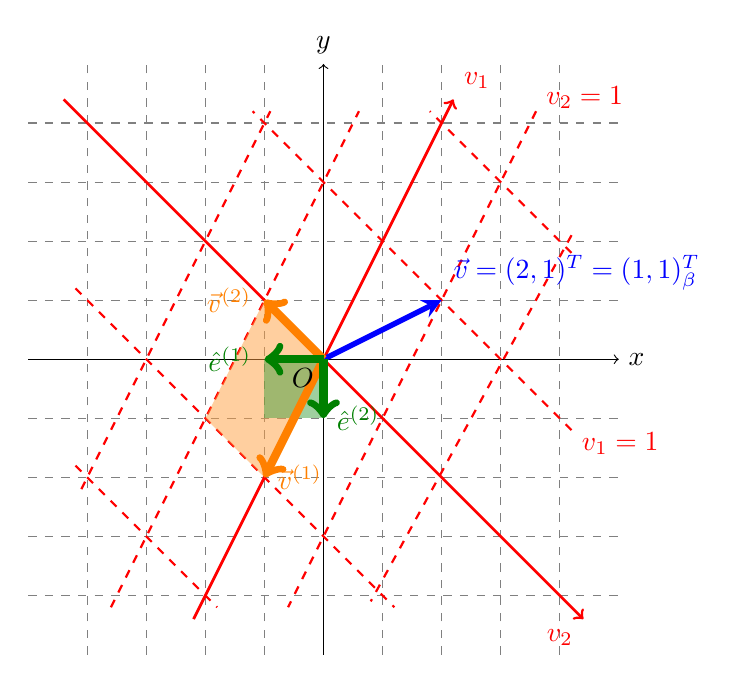
\begin{tikzpicture}[scale = 0.75]
\draw[->] (-5,0)--(5,0) node[right]{$x$};
\draw[->] (0,-5)--(0,5) node[above]{$y$};
\draw[gray,dashed] (-4,-5)--(-4,5);
\draw[gray,dashed] (-3,-5)--(-3,5);
\draw[gray,dashed] (-2,-5)--(-2,5);
\draw[gray,dashed] (-1,-5)--(-1,5);
\draw[gray,dashed] (4,-5)--(4,5);
\draw[gray,dashed] (3,-5)--(3,5);
\draw[gray,dashed] (2,-5)--(2,5);
\draw[gray,dashed] (1,-5)--(1,5);
\draw[gray,dashed] (-5,-4)--(5,-4);
\draw[gray,dashed] (-5,-3)--(5,-3);
\draw[gray,dashed] (-5,-2)--(5,-2);
\draw[gray,dashed] (-5,-1)--(5,-1);
\draw[gray,dashed] (-5,4)--(5,4);
\draw[gray,dashed] (-5,3)--(5,3);
\draw[gray,dashed] (-5,2)--(5,2);
\draw[gray,dashed] (-5,1)--(5,1);
\draw[red,->,line width=1] (-2.2,-4.4)--(2.2,4.4) node[above right]{$v_1$};
\draw[red,->,line width=1] (-4.4,4.4)--(4.4,-4.4) node[below left]{$v_2$};
\draw[red, thick, dashed] (4.2,-1.2)--(-1.2,4.2) node[right, pos=0, yshift=-5]{$v_1 = 1$};
\draw[red, thick, dashed] (3.6,4.2)--(-0.6,-4.2) node[right, pos=0, yshift=5]{$v_2 = 1$};
\draw[red, thick, dashed] (4.2,1.8)--(1.8,4.2);
\draw[red, thick, dashed] (4.2,2.1)--(0.8,-4.1);
\draw[red, thick, dashed] (-4.2,1.2)--(1.2,-4.2);
\draw[red, thick, dashed] (-4.2,-1.8)--(-1.8,-4.2);
\draw[red, thick, dashed] (-3.6,-4.2)--(0.6,4.2);
\draw[red, thick, dashed] (-4.1,-2.2)--(-0.9,4.2);
\draw[blue,-stealth,line width=2] (0,0)--(2,1) node[right, yshift=10]{$\vec{v} = (2,1)^T = (1,1)^T_\beta$};
\fill[orange!75, opacity=0.5] (0,0) -- (-1,1) -- (-2,-1) -- (-1,-2) -- cycle;
\fill[Green!75, opacity=0.5] (0,0) -- (-1,0) -- (-1,-1) -- (0,-1) -- cycle;
\draw[orange,->,line width=3] (0,0)--(-1,-2) node[right]{$\vec{v}^{(1)}$};
\draw[orange,->,line width=3] (0,0)--(-1,1) node[left]{$\vec{v}^{(2)}$};
\draw[Green,->,line width=3] (0,0)--(-1,0) node[left]{$\hat{e}^{(1)}$};
\draw[Green,->,line width=3] (0,0)--(0,-1) node[right]{$\hat{e}^{(2)}$};
\node[below left]{$O$}; 
\end{tikzpicture}
\caption{\textit{The geometry of Example \ref{exmp:2Dtransform}.}}
\label{fig:coordtransgeo}
\end{figure}
\end{solution}
In this example, we can see that in the two bases $\mathcal{S}$ and $\mathcal{\beta}$, their axis vectors (reversed in the figure) can be converted via $T: \mathbb{R}^2 \to \mathbb{R}^2$ with $T(\hat{e}^{(j)}) = \vec{v}^{(j)}$. The corresponding matrix representation is $\vec{v}^{(j)} = [\vec{v}^{(1)}|\vec{v}^{(2)}]\hat{e}^{(j)} = \smash{P_\beta^S}\hat{e}^{(j)}$. Meanwhile, the coordinate transformation of a fixed vector follows $[\vec{v}]_\beta = \smash{(P_\beta^S)^{-1}}[\vec{v}]_S = \smash{P_S^\beta}[\vec{v}]_S$, where the matrix involved is the inverse of the former. The former case actually alters the vectors themselves and is sometimes known as an \index{Active Transformation}\keywordhl{active (coordinate) transformation}. In contrast, the latter only changes the coordinate frame but keeps the vector unchanged physically and is hence called a \index{Passive Transformation}\keywordhl{passive (coordinate) transformation} (in fact, it is just the identity transformation with a change of basis). We can see that in the example above, after the active transformation, the area of the square formed by the new two basis vectors is enlarged by a factor of $\abs{\det(\smash{P_\beta^S})}=3$. It is a result of Properties \ref{proper:nvolume} and the similar holds for cases of any dimension. Oppositely, with the passive transformation we can say that the value of the area of an identical square is shrunk to $\abs{\det(\smash{P_S^\beta})} = \abs{\det(\smash{(P_\beta^S)^{-1}})} = \abs{\det(\smash{P_\beta^S})}^{-1} = \frac{1}{3}$ of the original, expressed in the new basis units. Therefore, the appropriate factors in the two scenarios are the reciprocal of each other.

\subsubsection{Change of Coordinates for Linear Transformations/Matrices}

It is also possible to do a change of coordinates for linear transformations and hence the matrices that represent them. Consider a linear transformation $T: \mathcal{U} \to \mathcal{V}$ that has a matrix representation of $[\vec{v}]_\eta = \smash{[T]_\beta^\eta}[\vec{u}]_\beta$ where $\mathcal{\beta}$ and $\mathcal{\eta}$ are bases for $\mathcal{U}$ and $\mathcal{V}$ respectively. If we want to change the basis for $\mathcal{U}$ from $\mathcal{\beta}$ to some other basis $\mathcal{\beta}'$ (and similarly $\mathcal{\eta}'$ for $\mathcal{V}$), then the new matrix representation of the linear transformation would be $[\vec{v}]_{\eta'} = \smash{[T]_{\beta'}^{\eta'}}[\vec{u}]_{\beta'}$. Since they are the same transformation but only expressed in different coordinate systems, these two matrix equations have to be equivalent. Now, the vectors on both sides of the original equation themselves can undergo changes of coordinates according to the previous Theorem \ref{thm:bijectivechincoord} with $[\vec{u}]_\beta = \smash{[\text{id}]_{\beta'}^\beta} [\vec{u}]_{\beta'} = \smash{P_{\beta'}^\beta} [\vec{u}]_{\beta'}$ and $[\vec{v}]_{\eta} = \smash{[\text{id}]_{\eta'}^{\eta}} [\vec{v}]_{\eta'} = \smash{Q_{\eta'}^\eta} [\vec{v}]_{\eta'}$, where we denote the coordinate transition matrix from $\mathcal{\beta'}$ to $\mathcal{\beta}$ by $\smash{P_{\beta'}^{\beta}}$ (and similarly $\mathcal{\eta'}$ to $\mathcal{\eta}$ by $\smash{Q_{\eta'}^{\eta}}$). Subsequently,
\begin{align*}
[\vec{v}]_\eta &= [T]_\beta^\eta[\vec{u}]_\beta \\
Q_{\eta'}^\eta [\vec{v}]_{\eta'} &= [T]_\beta^\eta P_{\beta'}^\beta [\vec{u}]_{\beta'} \\
[\vec{v}]_{\eta'} &= \left( (Q_{\eta'}^\eta)^{-1} [T]_\beta^\eta P_{\beta'}^\beta \right) [\vec{u}]_{\beta'}
\end{align*}
Comparing with the assumed form of $[\vec{v}]_{\eta'} = \smash{[T]_{\beta'}^{\eta'}}[\vec{u}]_{\beta'}$, we can identify $\smash{[T]_{\beta'}^{\eta'}}$ with $\smash{(Q_{\eta'}^\eta)^{-1} [T]_\beta^\eta P_{\beta'}^\beta}$, and this is the desired formula for change of coordinates over the matrix form of a linear transformation.
\begin{proper}
\label{proper:chcoordsmat}
The change of coordinates for the matrix representation of a linear transformation $T: \mathcal{U} \to \mathcal{V}$ from bases $\mathcal{\beta}$ and $\mathcal{\eta}$ to $\mathcal{\beta}'$ and $\mathcal{\eta}'$ for $\mathcal{U}$ and $\mathcal{V}$ respectively, follows the relation
\begin{align}
[T]_{\beta'}^{\eta'} = (Q_{\eta'}^\eta)^{-1} [T]_\beta^\eta P_{\beta'}^\beta \label{eqn:coordchangelintrans}
\end{align}
where $\smash{P_{\beta'}^{\beta}}$ and $\smash{Q_{\eta'}^{\eta}}$ are matrices for change of coordinates on vectors from $\mathcal{\beta'}$ to $\mathcal{\beta}$ and $\mathcal{\eta'}$ to $\mathcal{\eta}$ individually.
\end{proper}
Another way to derive the above formula is to consider the linear transformation with respect to the basis $\mathcal{\beta'}$ to $\mathcal{\eta'}$ as three smaller steps: firstly, convert the input vector from the basis $\mathcal{\beta'}$ back to $\mathcal{\beta}$ ($\smash{P_{\beta'}^\beta}$); subsequently, carry out the transformation in terms of $\mathcal{\beta}$ and $\mathcal{\eta}$ ($\smash{[T]_\beta^\eta}$); finally, map the vector from the basis $\mathcal{\eta}$ to $\mathcal{\eta'}$ ($\smash{Q_\eta^{\eta'} = (Q_{\eta'}^\eta)^{-1}}$). This flow is illustrated in the schematic of Figure \ref{fig:transcoordsmatrix}.
\begin{figure}[ht!]
    \centering
    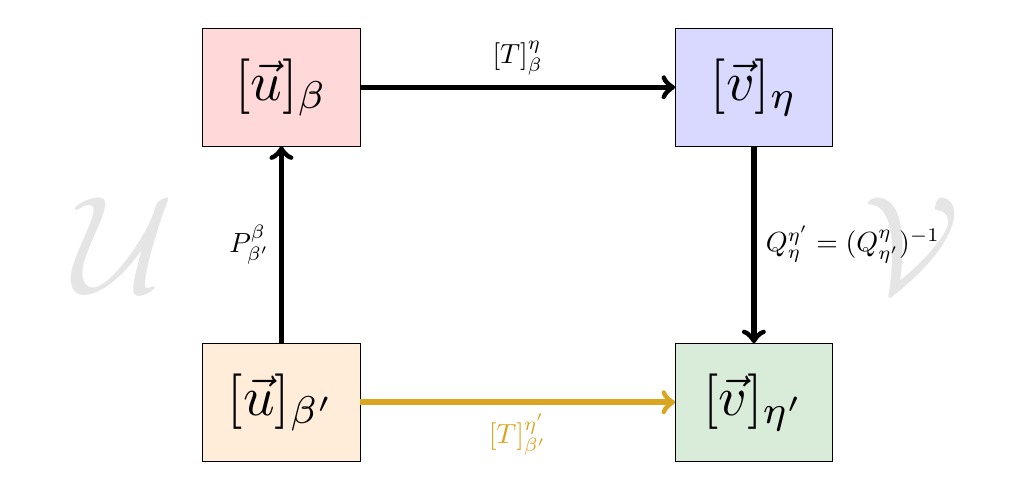
\begin{tikzpicture}
    \node[opacity=0.1,scale=5] at (-2,-2) {$\mathcal{U}$}; 
    \node[opacity=0.1,scale=5] at (8,-2) {$\mathcal{V}$};
    \draw [fill=red!15] (-1,-0.75) rectangle (1,0.75);
    \draw [fill=orange!15] (-1,-4.75) rectangle (1,-3.25);
    \draw [fill=blue!15] (5,-0.75) rectangle (7,0.75);
    \draw [fill=Green!15] (5,-4.75) rectangle (7,-3.25);
    \node[scale=2] at (0,0) {$[\vec{u}]_\beta$};
    \node[scale=2] at (6,0) {$[\vec{v}]_\eta$};
    \node[scale=2] at (0,-4) {$[\vec{u}]_{\beta'}$};
    \node[scale=2] at (6,-4) {$[\vec{v}]_{\eta'}$}; 
    \draw[->, line width=2] (0,-3.25) -- (0,-0.75) node[midway, left]{$P_{\beta'}^\beta$};
    \draw[->, line width=2] (6,-0.75) -- (6,-3.25) node[midway, right]{$Q_\eta^{\eta'} = (Q_{\eta'}^\eta)^{-1}$};
    \draw[->, line width=2] (1,0) -- (5,0) node[midway, above]{$[T]_\beta^\eta$};
    \draw[Goldenrod, ->, line width=2] (1,-4) -- (5,-4) node[midway, below]{$[T]_{\beta'}^{\eta'}$};
    \end{tikzpicture}
    \caption{\textit{A schematic showing how the change of coordinate bases works for linear transformation.}}
    \label{fig:transcoordsmatrix}
\end{figure}

\begin{exmp}
Use Properties \ref{proper:chcoordsmat} to redo Example \ref{exmp:lineartransderivative} with respect to new bases $\mathcal{\beta}' = \{1, x-1, (x-1)^2\}$ and $\mathcal{\eta}' = \{1, x+1\}$.
\end{exmp}
\begin{solution}
First it is instructive to find $\smash{P_{\beta'}^\beta}$ and $\smash{Q_{\eta'}^\eta}$. We leave it to the readers to verify that
\begin{align*}
P_{\beta'}^\beta &= 
\begin{bmatrix}
1 & -1 & 1 \\
0 & 1 & -2\\
0 & 0 & 1
\end{bmatrix}
& Q_{\eta'}^\eta &=
\begin{bmatrix}
1 & 1 \\
0 & 1 
\end{bmatrix}
\end{align*}
and hence by Properties \ref{proper:chcoordsmat},
\begin{align*}
[T]_{\beta'}^{\eta'} &= (Q_{\eta'}^\eta)^{-1} [T]_\beta^\eta P_{\beta'}^\beta \\
&= \begin{bmatrix}
1 & 1 \\
0 & 1 
\end{bmatrix}^{-1}
\begin{bmatrix}
0 & 1 & 0 \\
0 & 0 & 2
\end{bmatrix}
\begin{bmatrix}
1 & -1 & 1 \\
0 & 1 & -2\\
0 & 0 & 1
\end{bmatrix} \\
&= \begin{bmatrix}
1 & -1 \\
0 & 1 
\end{bmatrix}
\begin{bmatrix}
0 & 1 & 0 \\
0 & 0 & 2
\end{bmatrix}
\begin{bmatrix}
1 & -1 & 1 \\
0 & 1 & -2\\
0 & 0 & 1
\end{bmatrix} =
\begin{bmatrix}
0 & 1 & -4 \\
0 & 0 & 2
\end{bmatrix}
\end{align*}
We use a test case to check the answer. Let $p(x) = x^2 - 3x + 1 = (x-1)^2 - (x-1) - 1$. Then its coordinates in the $\mathcal{\beta}'$ basis is $(-1,-1,1)^T_{\beta'}$, and the transformation can be described by 
\begin{align*}
[T]_{\beta'}^{\eta'} (-1,-1,1)^T_{\beta'} &= 
\begin{bmatrix}
0 & 1 & -4 \\
0 & 0 & 2
\end{bmatrix}_{\beta'}^{\eta'}
\begin{bmatrix}
-1 \\
-1 \\
1
\end{bmatrix}_{\beta'}
=
\begin{bmatrix}
-5 \\
2
\end{bmatrix}_{\eta'}
\end{align*}
which corresponds to $-5(1) + 2(x+1) = 2x-3$, which is consistent with the usual calculation $T(p(x)) = p'(x) = (x^2-3x+1)' = 2x-3$ from elementary Calculus.
\end{solution}

Most of the time, we are interested in the type of linear transformations that are an \index{Endomorphism}\keywordhl{endomorphism} (sometimes also referred to as a \index{Linear Operator}\keywordhl{(linear) operator}) in which the mapping is from a vector space $\mathcal{V}$ to itself, i.e.\ $T: \mathcal{V} \to \mathcal{V}$\footnote{An endomorphism that is at the same time an isomorphism is known as an \index{Automorphism}\keywordhl{automorphism}, e.g.\ the linear transformation in Example \ref{exmp:endomorphch}.}. Often we also use the same basis $\mathcal{\beta}$ for the input and output vector. Subsequently, to change the basis for both of them at the same time, let's say $\mathcal{\beta}'$, if the matrix for change of coordinates on vectors from $\mathcal{\beta}'$ to $\mathcal{\beta}$ is denoted as $P = \smash{P_{\beta'}^\beta}$, then (\ref{eqn:coordchangelintrans}) of Properties \ref{proper:chcoordsmat} is reduced to $\smash{[T]_{\beta'}^{\beta'}} = \smash{(P_{\beta'}^\beta)^{-1} [T]_\beta^\beta P_{\beta'}^\beta} = P^{-1}AP$ where $A = \smash{[T]_\beta^\beta}$ is the original matrix representation of the endomorphism. When it is clear from the context, we will simply write $\smash{[T]_\beta^\beta}$ and $\smash{[T]_{\beta'}^{\beta'}}$ as $[T]_\beta$ and $[T]_{\beta'}$.
\begin{proper}
\label{proper:endomorph}
For a linear endomorphism/operator $T: \mathcal{V} \to \mathcal{V}$, the change of coordinates for its matrix representation from the old basis $\mathcal{\beta}$ to the new one $\mathcal{\beta}'$ is described by the formula
\begin{align}
[T]_{\beta'} = (P_{\beta'}^\beta)^{-1} [T]_\beta P_{\beta'}^\beta  \label{eqn:endomorphcoordch}  
\end{align}
\end{proper}
Speaking loosely, the change of coordinates for a matrix in general takes the form of
\begin{align}
A' = P^{-1}AP
\end{align}
In this case, $A'$ and $A$ (or $[T]_{\beta'}$ and $[T]_\beta$) are said to be \index{Similar}\keywordhl{similar}.

\begin{exmp}
\label{exmp:endomorphch}
For a two-dimensional vector space $\mathcal{V}$ with a basis $\mathcal{\beta} = \{\vec{v}^{(1)}, \vec{v}^{(2)}\}$, if a linear endomorphism $T: \mathcal{V} \to \mathcal{V}$ is defined by $T(\vec{v}^{(1)}) = \vec{v}^{(1)}$, $T(\vec{v}^{(2)}) = \vec{v}^{(1)} + \vec{v}^{(2)}$, finds its matrix representation with respect to $\mathcal{\beta}$. Subsequently, if a new basis $\mathcal{\beta}'$ is formed by $\{\vec{v}^{(1)'}, \vec{v}^{(2)'}\}$ where $\vec{v}^{(1)'} = 2\vec{v}^{(1)} - \vec{v}^{(2)}$ and $\vec{v}^{(2)'} = -\vec{v}^{(1)} + \vec{v}^{(2)}$, use Properties \ref{proper:endomorph} to compute the matrix representation of the endomorphism with respect to the new basis.
\end{exmp}
\begin{solution}
By Definition \ref{defn:matrixrepoflintrans}, the linear transformation has a matrix representation of
\begin{align*}
[T]_\beta = \begin{bmatrix}
[T(\vec{v}^{(1)})]_\beta|[T(\vec{v}^{(2)})]_\beta    
\end{bmatrix} &= 
\begin{bmatrix}
[\vec{v}^{(1)}]_\beta|[\vec{v}^{(1)} + \vec{v}^{(2)}]_\beta    
\end{bmatrix} \\
&=
\begin{bmatrix}
1 & 1 \\
0 & 1
\end{bmatrix}
\end{align*}
with respect to the old basis $\mathcal{\beta}$. The appropriate $\smash{P_{\beta'}^\beta}$ matrix that will be used for Properties \ref{proper:endomorph}, by (\ref{eqn:PBB'}), is
\begin{align*}
P_{\beta'}^\beta = 
\begin{bmatrix}
[\vec{v}^{(1)'}]_\beta|[\vec{v}^{(2)'}]_\beta
\end{bmatrix}
&= \begin{bmatrix}
[2\vec{v}^{(1)} - \vec{v}^{(2)}]_\beta|[-\vec{v}^{(1)} + \vec{v}^{(2)}]_\beta
\end{bmatrix} \\
&=
\begin{bmatrix}
2 & -1 \\
-1 & 1
\end{bmatrix}
\end{align*}
and thus by (\ref{eqn:endomorphcoordch}) the desired new matrix representation of the endomorphism with respect to $\mathcal{\beta}'$ is
\begin{align*}
[T]_{\beta'} &= (P_{\beta'}^\beta)^{-1} [T]_\beta P_{\beta'}^\beta \\
&= 
\begin{bmatrix}
2 & -1 \\
-1 & 1
\end{bmatrix}^{-1}
\begin{bmatrix}
1 & 1 \\
0 & 1
\end{bmatrix}
\begin{bmatrix}
2 & -1 \\
-1 & 1
\end{bmatrix} \\
&= 
\begin{bmatrix}
1 & 1 \\
1 & 2
\end{bmatrix}
\begin{bmatrix}
1 & 1 \\
0 & 1
\end{bmatrix}
\begin{bmatrix}
2 & -1 \\
-1 & 1
\end{bmatrix}
=
\begin{bmatrix}
0 & 1\\
-1 & 2
\end{bmatrix}
\end{align*}
\end{solution}

\subsection{Gram-Schmidt Orthogonalization, QR Decomposition}
\label{section:GSortho}
Sometimes the coordinate basis consists of vectors that are linearly independent but not orthogonal to each other, unlike the standard basis. A common way to create an orthogonal basis from the set is to apply the so-called \index{Gram-Schmidt Orthogonalization}\keywordhl{Gram-Schmidt Orthogonalization}. Basically, it is an iterative method. At each step, it constructs a vector that is orthogonal to all the previously processed vectors by removing the parallel components projected onto them (blue in Figure \ref{fig:7.3}) while retaining the orthogonal part (red).
\begin{figure}[ht!]
\centering
\begin{tikzpicture}[scale=1.3]
\coordinate (0) at (0,0);
\coordinate (vecu) at (4,1);
\coordinate (vecv) at (1,2);
\draw[->](0)--(vecu) node[right]{$\vec{u}^{(1)}$, $\vec{v}^{(1)}$};
\draw[->](0)--(vecv) node[above]{$\vec{u}^{(2)}$};
\draw[red, dashed, thick, ->] (24/17, 6/17)--(1,2) node[midway, right]{$\vec{v^{(2)}}$};
\draw[red] (24/17+0.2, 6/17+0.05)--(24/17+0.15, 6/17+0.25)--(24/17-0.05, 6/17+0.2);
\pic[draw, "$\theta$", angle eccentricity=1.5] {angle = vecu--0--vecv};
\draw[blue, very thick] (0,0)--(24/17, 6/17) node[below, shift={(0mm, -2mm)}]{$\text{proj}_{v^{(1)}}\vec{u}^{(2)}$};
\end{tikzpicture}
\caption{\textit{Similar to Figure \ref{fig:dotproj} but with the parallel and orthogonal components of the projection highlighted.}}
\label{fig:7.3}
\end{figure}
\begin{defn}[Algorithm for Gram-Schmidt Orthogonalization]
\label{defn:GSorth}
Given a coordinate basis consisted of $\vec{u}^{(1)}, \vec{u}^{(2)}, \vec{u}^{(3)}, \ldots, \vec{u}^{(n)} \in \mathbb{R}^m$, Gram-Schmidt Orthogonalization transforms them into an orthogonal one with $\vec{v}^{(1)}, \vec{v}^{(2)}, \vec{v}^{(3)}, \ldots, \vec{v}^{(n)} \in \mathbb{R}^m$ ($m$ and $n$ are not necessarily equal, specifically $n \leq m$) according to the following formulae:
\begin{align}
\vec{v}^{(1)} &= \vec{u}^{(1)} \nonumber \\
\vec{v}^{(2)} &= \vec{u}^{(2)} - \text{proj}_{v^{(1)}}\vec{u}^{(2)} = \vec{u}^{(2)} - \frac{\vec{u}^{(2)} \cdot \vec{v}^{(1)}}{\norm{\vec{v}^{(1)}}^2} \vec{v}^{(1)} \nonumber \\
\vec{v}^{(3)} &= \vec{u}^{(3)} - \text{proj}_{v^{(1)}}\vec{u}^{(3)} - \text{proj}_{v^{(2)}}\vec{u}^{(3)} \\
&= \vec{u}^{(3)} - \frac{\vec{u}^{(3)} \cdot \vec{v}^{(1)}}{\norm{\vec{v}^{(1)}}^2} \vec{v}^{(1)} - \frac{\vec{u}^{(3)} \cdot \vec{v}^{(2)}}{\norm{\vec{v}^{(2)}}^2} \vec{v}^{(2)} \nonumber \\
\vdots \nonumber \\
\vec{v}^{(n)} &= \vec{u}^{(n)} - \text{proj}_{v^{(1)}}\vec{u}^{(n)} - \text{proj}_{v^{(2)}}\vec{u}^{(n)} - \cdots - \text{proj}_{v^{(n-1)}}\vec{u}^{(n)} \nonumber \\
&= \vec{u}^{(n)} - \frac{\vec{u}^{(n)} \cdot \vec{v}^{(1)}}{\norm{\vec{v}^{(1)}}^2} \vec{v}^{(1)} - \frac{\vec{u}^{(n)} \cdot \vec{v}^{(2)}}{\norm{\vec{v}^{(2)}}^2} \vec{v}^{(2)} - \cdots - \frac{\vec{u}^{(n)} \cdot \vec{v}^{(n-1)}}{\norm{\vec{v}^{(n-1)}}^2} \vec{v}^{(n-1)} \nonumber
\end{align}
In general, for $j \geq 2$, the $j$-th new vector is computed by
\begin{align}
\vec{v}^{(j)} &= \vec{u}^{(j)} - \sum_{k=1}^{j-1}\text{proj}_{v^{(k)}}\vec{u}^{(j)}  = \vec{u}^{(j)} - \sum_{k=1}^{j-1}\frac{\vec{u}^{(j)} \cdot \vec{v}^{(k)}}{\norm{\vec{v}^{(k)}}^2} \vec{v}^{(k)}
\end{align}
where the expression of vector projection, Properties \ref{proper:proj}, is used.
\end{defn}
A variant of Gram-Schmidt Orthogonalization is to normalize every vector at each step immediately, such that $\norm{\hat{v}^{(j)}} = 1$ for all $j$, and the resulting basis is said to be \index{Orthonormal}\keywordhl{orthonormal} (both orthogonal and of unit length). The formulae in Definition \ref{defn:GSorth} are then reduced to
\begin{defn}[Gram-Schmidt Orthogonalization with Normalization]
\label{defn:GSorth_norm}
\begin{align}
\hat{v}^{(1)} &= \frac{\vec{u}^{(1)}}{\norm{\vec{u}^{(1)}}} \nonumber \\
\hat{v}^{(2)} &= \frac{\vec{u}^{(2)} - (\vec{u}^{(2)} \cdot \hat{v}^{(1)})\hat{v}^{(1)}}{\norm{\vec{u}^{(2)} - (\vec{u}^{(2)} \cdot \hat{v}^{(1)})\hat{v}^{(1)}}} \nonumber \\
\hat{v}^{(3)} &= \frac{\vec{u}^{(3)} - (\vec{u}^{(3)} \cdot \hat{v}^{(1)})\hat{v}^{(1)} - (\vec{u}^{(3)} \cdot \hat{v}^{(2)})\hat{v}^{(2)}}{\norm{\vec{u}^{(3)} - (\vec{u}^{(3)} \cdot \hat{v}^{(1)})\hat{v}^{(1)} - (\vec{u}^{(3)} \cdot \hat{v}^{(2)})\hat{v}^{(2)}}} \\
\vdots \nonumber \\
\hat{v}^{(n)} &= \frac{\vec{u}^{(n)} - (\vec{u}^{(n)} \cdot \hat{v}^{(1)})\hat{v}^{(1)} - (\vec{u}^{(n)} \cdot \hat{v}^{(2)})\hat{v}^{(2)} - \cdots - (\vec{u}^{(n)} \cdot \hat{v}^{(n-1)})\hat{v}^{(n-1)}}{\norm{\vec{u}^{(n)} - (\vec{u}^{(n)} \cdot \hat{v}^{(1)})\hat{v}^{(1)} - (\vec{u}^{(n)} \cdot \hat{v}^{(2)})\hat{v}^{(2)} - \cdots - (\vec{u}^{(n)} \cdot \hat{v}^{(n-1)})\hat{v}^{(n-1)}}} \nonumber
\end{align}
For $j \geq 2$, the general formula is
\begin{align}
\hat{v}^{(j)} &= \frac{\vec{u}^{(j)} - \sum_{k=1}^{j-1}(\vec{u}^{(j)} \cdot \hat{v}^{(k)})\hat{v}^{(k)}}{\norm{\vec{u}^{(j)} - \sum_{k=1}^{j-1}(\vec{u}^{(j)} \cdot \hat{v}^{(k)})\hat{v}^{(k)}}} \label{eqn:GSorth_norm}
\end{align}
\end{defn}
\begin{exmp}
\label{exmp:GS_ex}
Perform Gram-Schmidt Orthogonalization with normalization on the coordinate basis for $\mathbb{R}^3$ that is consisted of $\vec{u}^{(1)} = (1,2,2)^T$, $\vec{u}^{(2)} = (1,-1,0)^T$, $\vec{u}^{(3)} = (3,-1,1)^T$, using the formulae in Definition \ref{defn:GSorth_norm}.
\end{exmp}
\begin{solution}
The first vector is
\begin{align*}
\hat{v}^{(1)} &= \frac{1}{\sqrt{1^2+2^2+2^2}}
\begin{bmatrix}
1 \\
2 \\
2
\end{bmatrix} 
= 
\frac{1}{3}
\begin{bmatrix}
1 \\
2 \\
2
\end{bmatrix} 
=
\begin{bmatrix}
\frac{1}{3} \\
\frac{2}{3} \\
\frac{2}{3}
\end{bmatrix}
\end{align*}
The second vector can be found via
\begin{align*}
&\quad \vec{u}^{(2)} - (\vec{u}^{(2)} \cdot \hat{v}^{(1)})\hat{v}^{(1)} \\
&= 
\begin{bmatrix}
1 \\
-1 \\
0
\end{bmatrix} 
-
\left[(1)(\frac{1}{3}) + (-1)(\frac{2}{3}) + (0)(\frac{2}{3})\right]
\begin{bmatrix}
\frac{1}{3} \\
\frac{2}{3} \\
\frac{2}{3}
\end{bmatrix} \\
&= 
\begin{bmatrix}
1 \\
-1 \\
0
\end{bmatrix}
- (-\frac{1}{3})
\begin{bmatrix}
\frac{1}{3} \\
\frac{2}{3} \\
\frac{2}{3}
\end{bmatrix}
=
\begin{bmatrix}
\frac{10}{9} \\
-\frac{7}{9} \\
\frac{2}{9}
\end{bmatrix} \\
\hat{v}^{(2)} &= \frac{1}{\sqrt{(\frac{10}{9})^2+(-\frac{7}{9})^2+(\frac{2}{9})^2}}
\begin{bmatrix}
\frac{10}{9} \\
-\frac{7}{9} \\
\frac{2}{9}
\end{bmatrix}
=
\frac{3}{\sqrt{17}}
\begin{bmatrix}
\frac{10}{9} \\
-\frac{7}{9} \\
\frac{2}{9}
\end{bmatrix}
=
\begin{bmatrix}
\frac{10}{3\sqrt{17}} \\
-\frac{7}{3\sqrt{17}}\\
\frac{2}{3\sqrt{17}}
\end{bmatrix}
\end{align*}
By the same essence, we have the third vector as
\begin{align*}
&\quad \vec{u}^{(3)} - (\vec{u}^{(3)} \cdot \hat{v}^{(1)})\hat{v}^{(1)} - (\vec{u}^{(3)} \cdot \hat{v}^{(2)})\hat{v}^{(2)}\\
&=
\begin{bmatrix}
3 \\
-1 \\
1
\end{bmatrix}
-
\left[(3)(\frac{1}{3}) + (-1)(\frac{2}{3}) + (1)(\frac{2}{3})\right]
\begin{bmatrix}
\frac{1}{3} \\
\frac{2}{3} \\
\frac{2}{3}
\end{bmatrix} \\
&\quad -
\left[(3)(\frac{10}{3\sqrt{17}}) + (-1)(-\frac{7}{3\sqrt{17}}) + (1)(\frac{2}{3\sqrt{17}})\right]
\begin{bmatrix}
\frac{10}{3\sqrt{17}} \\
-\frac{7}{3\sqrt{17}} \\
\frac{2}{3\sqrt{17}}
\end{bmatrix} \\
&=
\begin{bmatrix}
3 \\
-1 \\
1
\end{bmatrix}
- 1
\begin{bmatrix}
\frac{1}{3} \\
\frac{2}{3} \\
\frac{2}{3}
\end{bmatrix}
-
\textcolor{red}{\frac{13}{\sqrt{17}}}
\begin{bmatrix}
\frac{10}{3\sqrt{17}} \\
-\frac{7}{3\sqrt{17}} \\
\frac{2}{3\sqrt{17}}
\end{bmatrix}
=
\begin{bmatrix}
\frac{2}{17} \\
\frac{2}{17} \\
-\frac{3}{17}
\end{bmatrix}
\\
\hat{v}^{(3)} &= \frac{1}{\sqrt{(\frac{2}{17})^2 + (\frac{2}{17})^2 + (-(\frac{3}{17}))^2}}
\begin{bmatrix}
\frac{2}{17} \\
\frac{2}{17} \\
-\frac{3}{17}
\end{bmatrix}
=
\textcolor{blue}{\sqrt{17}}
\begin{bmatrix}
\frac{2}{17} \\
\frac{2}{17} \\
-\frac{3}{17}
\end{bmatrix}
=
\begin{bmatrix}
\frac{2}{\sqrt{17}} \\
\frac{2}{\sqrt{17}} \\
-\frac{3}{\sqrt{17}}
\end{bmatrix}
\end{align*}
\end{solution}
$\blacktriangleright$ Short Exercise: Verify that $\hat{v}^{(1)}, \hat{v}^{(2)}, \hat{v}^{(3)}$ are pairwise orthogonal.\footnotemark\par
A major application of the Gram-Schmidt Orthogonalization is the \index{QR Decomposition}\keywordhl{QR Decomposition}, which factors a matrix into two matrices, one as the orthogonal basis vectors acquired from the Gram-Schmidt process arranged in columns and another one as an upper-triangular matrix (non-zero entries only found along or above the main diagonal) where the entries take the form of $\vec{u}^{(j)} \cdot \hat{v}^{(i)}$ as shown below. This is very useful in the processing of large matrices and least-square error fitting.
\begin{proper}
\label{proper:QRdecompose}
For a matrix $A = [\vec{u}^{(1)}|\vec{u}^{(2)}|\vec{u}^{(3)}|\cdots|\vec{u}^{(n)}]$, and the matrix $Q = [\hat{v}^{(1)}|\hat{v}^{(2)}|\hat{v}^{(3)}|\cdots|\hat{v}^{(n)}]$, where the $\hat{v}^{(j)} \in \mathbb{R}^m$ are orthonormal vectors that come from carrying out Gram-Schmidt orthogonalization on the basis vectors $\vec{u}^{(j)} \in \mathbb{R}^m$, $m \geq n$, and $j = 1,2,\ldots,n$, according to the Definition \ref{defn:GSorth_norm}, we have $A = QR$, where
\begin{align}
R &= 
\begin{bmatrix}
\vec{u}^{(1)} \cdot \hat{v}^{(1)} & \vec{u}^{(2)} \cdot \hat{v}^{(1)} & \vec{u}^{(3)} \cdot \hat{v}^{(1)} & \cdots & \vec{u}^{(n)} \cdot \hat{v}^{(1)} \\
0 & \vec{u}^{(2)} \cdot \hat{v}^{(2)} & \vec{u}^{(3)} \cdot \hat{v}^{(2)} &  & \vec{u}^{(n)} \cdot \hat{v}^{(2)} \\
0 & 0 & \vec{u}^{(3)} \cdot \hat{v}^{(3)} &  & \vec{u}^{(n)} \cdot \hat{v}^{(3)} \\
\vdots & & & \ddots & \vdots\\
0 & 0 & 0 & \cdots & \vec{u}^{(n)} \cdot \hat{v}^{(n)} \\
\end{bmatrix} \label{eqn:QRR} \\
\text{i.e.\ } R_{ij} &= 
\begin{cases}
\vec{u}^{(j)} \cdot \hat{v}^{(i)} & i \leq j \\
0 & i > j
\end{cases}
& \text{for $1 \leq i, j \leq n$} \nonumber
\end{align}
is an upper-triangular $n \times n$ invertible matrix.
\end{proper}
\footnotetext{We will only check $\hat{v}^{(1)}$ and $\hat{v}^{(3)}$ are orthogonal to each other and leave the remaining two pairs to the readers. $\hat{v}^{(1)} \cdot \hat{v}^{(3)} = \smash{(\frac{1}{3}, \frac{2}{3}, \frac{2}{3})}^T \cdot \smash{(\frac{2}{\sqrt{17}}, \frac{2}{\sqrt{17}}, -\frac{3}{\sqrt{17}})}^T = \smash{(\frac{1}{3})(\frac{2}{\sqrt{17}})} + \smash{(\frac{2}{3})(\frac{2}{\sqrt{17}})} + \smash{(\frac{2}{3})(-\frac{3}{\sqrt{17}})} = 0$.}
\begin{proof}
We will show that every column of $A$ and $QR$ coincides. The $j$-th column of $A$ is simply the $j$-th vector in the starting basis, $\vec{u}^{(j)}$. Meanwhile, the $j$-th column of $QR$ is $Q$ times the $j$-th column of $R$, which is
\begin{align*}
QR^{(j)} &=
\begin{bmatrix}
\hat{v}^{(1)}|\hat{v}^{(2)}|\cdots|\hat{v}^{(j)}|\cdots|\hat{v}^{(n)}   
\end{bmatrix}
\begin{bmatrix}
\vec{u}^{(j)} \cdot \hat{v}^{(1)} \\   
\vec{u}^{(j)} \cdot \hat{v}^{(2)} \\   
\vdots \\
\vec{u}^{(j)} \cdot \hat{v}^{(j)} \\
\vdots \\
0
\end{bmatrix} \\
&= (\vec{u}^{(j)} \cdot \hat{v}^{(1)}) \hat{v}^{(1)} + (\vec{u}^{(j)} \cdot \hat{v}^{(2)}) \hat{v}^{(2)} + \cdots + (\vec{u}^{(j)} \cdot \hat{v}^{(j)}) \hat{v}^{(j)} + 0 \\
&= \sum_{k=1}^{j}(\vec{u}^{(j)} \cdot \hat{v}^{(k)})\hat{v}^{(k)} = \sum_{k=1}^{j-1}(\vec{u}^{(j)} \cdot \hat{v}^{(k)})\hat{v}^{(k)} + (\vec{u}^{(j)} \cdot \hat{v}^{(j)})\hat{v}^{(j)}
\end{align*}
By (\ref{eqn:GSorth_norm}) from Definition \ref{defn:GSorth_norm}, we have
\begin{align*}
\hat{v}^{(j)} &= \frac{\vec{u}^{(j)} - \sum_{k=1}^{j-1}(\vec{u}^{(j)} \cdot \hat{v}^{(k)})\hat{v}^{(k)}}{\norm{\vec{u}^{(j)} - \sum_{k=1}^{j-1}(\vec{u}^{(j)} \cdot \hat{v}^{(k)})\hat{v}^{(k)}}}
\end{align*}
\footnotemark{} which after rearrangement, becomes
\begin{align*}
\vec{u}^{(j)} = \sum_{k=1}^{j-1}(\vec{u}^{(j)} \cdot \hat{v}^{(k)})\hat{v}^{(k)} + {\norm{\vec{u}^{(j)} - \sum_{k=1}^{j-1}(\vec{u}^{(j)} \cdot \hat{v}^{(k)})\hat{v}^{(k)}}}\hat{v}^{(j)}
\end{align*}
Therefore, in order to show that $\vec{u}^{(j)} = QR^{(j)}$, by comparing the two expressions, we need to check if
\begin{align*}
\vec{u}^{(j)} \cdot \hat{v}^{(j)} &= \norm{\vec{u}^{(j)} - \sum_{k=1}^{j-1}(\vec{u}^{(j)} \cdot \hat{v}^{(k)})\hat{v}^{(k)}}
\end{align*}
Consider
\begin{align*}
\left[\vec{u}^{(j)} - \sum_{k=1}^{j-1}(\vec{u}^{(j)} \cdot \hat{v}^{(k)})\hat{v}^{(k)}\right] \cdot \hat{v}^{(j)} &= \vec{u}^{(j)} \cdot \hat{v}^{(j)} - \sum_{k=1}^{j-1}(\vec{u}^{(j)} \cdot \hat{v}^{(k)}) (\hat{v}^{(k)} \cdot \hat{v}^{(j)})\\
&= \vec{u}^{(j)} \cdot \hat{v}^{(j)}
\end{align*}
as $\hat{v}^{(k)} \cdot \hat{v}^{(j)} = 0$ for $k \neq j$ due to the orthogonality enforced by the Gram-Schmidt process. On the other hand, by Definition \ref{defn:GSorth_norm} again, 
\begin{align*}
\vec{u}^{(j)} - \sum_{k=1}^{j-1}(\vec{u}^{(j)} \cdot \hat{v}^{(k)})\hat{v}^{(k)} = \norm{\vec{u}^{(j)} - \sum_{k=1}^{j-1}(\vec{u}^{(j)} \cdot \hat{v}^{(k)})\hat{v}^{(k)}} \hat{v}^{(j)}
\end{align*}
Therefore,\footnotetext{\label{foot:GSnonzero} Some may ask if $\norm{\smash{\vec{u}^{(j)} - \sum_{k=1}^{j-1}(\vec{u}^{(j)} \cdot \hat{v}^{(k)})\hat{v}^{(k)}}}$ can be $0$ (or $\vec{u}^{(j)} - \sum_{k=1}^{j-1}(\vec{u}^{(j)} \cdot \hat{v}^{(k)})\hat{v}^{(k)}$ be the zero vector) and $\hat{v}^{(j)}$ is not well-defined. However, this will contradict the linear independence of the basis vectors $\vec{u}^{(k)}$, as each of $\hat{v}^{(k)}$ is a linear combination of $\vec{u}^{(1)}, \vec{u}^{(2)}, \ldots, \vec{u}^{(k)}$, deduced inductively from $k = 1$ to $k = j-1$ by looking at Definition \ref{defn:GSorth_norm}. Hence $\vec{u}^{(j)} - \smash{\sum_{k=1}^{j-1}(\vec{u}^{(j)} \cdot \hat{v}^{(k)})\hat{v}^{(k)}} = \textbf{0}$ implies a non-trivial solution to $\smash{c_1 \vec{u}^{(1)}} + \cdots + \smash{c_{j-1}\vec{u}^{(j-1)}} + \smash{c_j\vec{u}^{(j)}} = \textbf{0}$ where particularly $c_j = 1 \neq 0$.}
\begin{align*}
\left[\vec{u}^{(j)} - \sum_{k=1}^{j-1}(\vec{u}^{(j)} \cdot \hat{v}^{(k)})\hat{v}^{(k)}\right] \cdot \hat{v}^{(j)} &= \left(\norm{\vec{u}^{(j)} - \sum_{k=1}^{j-1}(\vec{u}^{(j)} \cdot \hat{v}^{(k)})\hat{v}^{(k)}} \hat{v}^{(j)}\right) \cdot \hat{v}^{(j)} \\
&= \norm{\vec{u}^{(j)} - \sum_{k=1}^{j-1}(\vec{u}^{(j)} \cdot \hat{v}^{(k)})\hat{v}^{(k)}} (\hat{v}^{(j)} \cdot\hat{v}^{(j)}) \\
&= \norm{\vec{u}^{(j)} - \sum_{k=1}^{j-1}(\vec{u}^{(j)} \cdot \hat{v}^{(k)})\hat{v}^{(k)}}
\end{align*}
as $\hat{v}^{(j)} \cdot \hat{v}^{(j)} = \norm{\hat{v}^{(j)}}^2 = 1$. The required equality is then established and the result follows. The invertibility of $R$ can be shown by noting that all diagonal components $\vec{u}^{(j)} \cdot \hat{v}^{(j)} = \norm{\smash{\vec{u}^{(j)} - \sum_{k=1}^{j-1}(\vec{u}^{(j)} \cdot \hat{v}^{(k)})\hat{v}^{(k)}}} $ of the upper-triangular $R$ matrix are non-zero (see Footnote \ref{foot:GSnonzero}). 
\end{proof}

\begin{exmp}
\label{exmp:QRdecom}
Construct a QR decomposition for the case in Example \ref{exmp:GS_ex}.
\end{exmp}
\begin{solution}
The matrix $Q$ simply consists of the orthonormal basis vectors:
\begin{align*}
Q &= 
\begin{bmatrix}
\frac{1}{3} & \frac{10}{3\sqrt{17}} & \frac{2}{\sqrt{17}} \\
\frac{2}{3} & -\frac{7}{3\sqrt{17}} & \frac{2}{\sqrt{17}} \\
\frac{2}{3} & \frac{2}{3\sqrt{17}} & -\frac{3}{\sqrt{17}}
\end{bmatrix}
\end{align*}
And by (\ref{eqn:QRR}) in Properties \ref{proper:QRdecompose}, the entries in $R$ are
\begin{align*}
R &= 
\begin{bmatrix}
\vec{u}^{(1)} \cdot \hat{v}^{(1)} & \vec{u}^{(2)} \cdot \hat{v}^{(1)} & \vec{u}^{(3)} \cdot \hat{v}^{(1)} \\
0 & \vec{u}^{(2)} \cdot \hat{v}^{(2)} & \vec{u}^{(3)} \cdot \hat{v}^{(2)} \\
0 & 0 & \vec{u}^{(3)} \cdot \hat{v}^{(3)}
\end{bmatrix}  \\
&= 
\begin{bmatrix}
3 & -\frac{1}{3} & 1 \\
0 & \frac{\sqrt{17}}{3} & \textcolor{red}{\frac{13}{\sqrt{17}}}  \\
0 & 0 & \textcolor{blue}{\frac{1}{\sqrt{17}}} \\
\end{bmatrix} 
\end{align*}
whose values can be readily inferred from the steps during the orthogonalization process itself in Example \ref{exmp:GS_ex} (highlighted in red/blue). The readers are encouraged to compute the matrix product $QR$ to see if the original matrix $A$ is recovered.
\end{solution}
We conclude this section with two small remarks, one related to computing the coordinates relative to an orthonormal basis, and another related to the concept of orthogonal complement discussed at the end of Section \ref{section:null}.
\begin{proper}
\label{proper:orthocoords}
The coordinates of a vector $\vec{v}$ in an orthonormal coordinate system $\beta$ are simply its dot products (projections onto) with the orthonormal basis vectors in $\beta$.
\end{proper}
\begin{proof}
As $\beta$ is an orthonormal coordinate system, according to the discussion in Section \ref{section:subspacebasis}, $\vec{v}$ can be written as a unique linear combination of the orthonormal basis vectors \smash{$\vec{v} = [v_1]_\beta \hat{e}_\beta^{(1)} + [v_2]_\beta \hat{e}_\beta^{(2)} + \cdots + [v_n]_\beta \hat{e}_\beta^{(n)}$}. By taking the dot product with \smash{$\hat{e}_\beta^{(1)}$}, we have
\begin{align*}
\vec{v} \cdot \hat{e}_\beta^{(1)} &= [v_1]_\beta (\hat{e}_\beta^{(1)} \cdot \hat{e}_\beta^{(1)}) + [v_2]_\beta (\hat{e}_\beta^{(2)} \cdot \hat{e}_\beta^{(1)}) + \cdots + [v_n]_\beta (\hat{e}_\beta^{(n)} \cdot \hat{e}_\beta^{(1)}) \\
&= [v_1]_\beta (1) + [v_2]_\beta (0) + \cdots + [v_n]_\beta (0) \\
&\quad \text{(Orthonormality of the basis vectors)} \\
&= [v_1]_\beta
\end{align*}
which is also the projection of $\vec{v}$ onto \smash{$\hat{e}_\beta^{(1)}$} by Properties \ref{proper:proj}. The same applies to the other coordinate components.
\end{proof}
\begin{proper}
\label{proper:orthodirectsum}
For an orthogonal(-normal) basis $\mathcal{\beta} = \{\vec{v}^{(1)}, \vec{v}^{(2)}, \vec{v}^{(3)}, \cdots, \allowbreak \vec{v}^{(n)}\}$ for a finite, $n$-dimensional vector space $\mathcal{V}$, the subspaces $\mathcal{V}_\gamma$ and $\mathcal{V}_\eta$ formed by $\mathcal{\gamma} = \{\vec{v}^{(I)}\}$ and $\mathcal{\eta} = \{\vec{v}^{(J)}\}$ respectively, where $I$ and $J$ are mutually exclusive indices that together count all integers from $1$ to $n$, are the orthogonal complement to each other with respect to $\mathcal{V}$, such that $\mathcal{V}_\gamma^\perp = \mathcal{V}_\eta$ ($\mathcal{V}_\eta^\perp = \mathcal{V}_\gamma$) and $\mathcal{V}_\gamma \oplus \mathcal{V}_\eta = \mathcal{V}$.
\end{proper}

\section{Python Programming}
We can define a function for a change in coordinates for vectors or matrices. Let's first write a helper function to produce the change of coordinates matrix $P$ proposed in Theorem \ref{thm:bijectivechincoord}, which is equal to $B'^{-1}B$ as discussed at the end of Example \ref{exmp:changecoord}:
\begin{lstlisting}
import numpy as np
from scipy import linalg

def P_matrix(B, B_prime):
    """ Computes the P matrix of change in coordinates. """
    P = linalg.inv(B_prime) @ B
    return(P)
\end{lstlisting}
Then we use Example \ref{exmp:2Dtransform} as an illustration for coordinate change for vectors, where regarding $\mathcal{\beta}$, we have
\begin{align*}
B = 
\begin{bmatrix}
1 & 1 \\ 
2 & -1
\end{bmatrix}
\end{align*}
and $B' = I$ as $\mathcal{\beta}' = \mathcal{S}$ implicitly in this case. We define another function for transforming the coordinates of any given vector as
\begin{lstlisting}
def coord_trans_vector(vec, P):
    """ Transforms the coordinates of a vector. """
    trans_vec = linalg.inv(P) @ vec
    return(trans_vec)
\end{lstlisting}
Then, Example \ref{exmp:2Dtransform} can be proceeded as follows.
\begin{lstlisting}
B1 = np.array([[1.,  1.], 
              [2., -1.]])

P1 = P_matrix(B1, np.identity(2))
old_v = np.array([2., 1.])
new_v = coord_trans_vector(old_v, P1)
print(new_v)
\end{lstlisting}
which returns \verb|[1. 1.]| correctly. Similarly, according to Properties \ref{proper:endomorph}, we can make a function to carry out the change of coordinates for matrices through
\begin{lstlisting}
def coord_trans_matrix(A, P):
    """ Transforms the coordinates of a matrix. """
    trans_matrix = linalg.inv(P) @ A @ P
    return(trans_matrix)
\end{lstlisting}
Let's use this to redo Example \ref{exmp:endomorphch}, where
\begin{align*}
A &= 
\begin{bmatrix}
1 & 1 \\
0 & 1
\end{bmatrix} &
& P=
\begin{bmatrix}
2 & -1 \\
-1 & 1
\end{bmatrix}
\end{align*}
Subsequently,
\begin{lstlisting}
B2 = np.array([[2., -1.], 
             [-1.,  1.]])
old_A = np.array([[1.,  1.], 
              [0.,  1.]])

P2 = P_matrix(B2, np.identity(2))
new_A = coord_trans_matrix(old_A, P2)
print(new_A)
\end{lstlisting}
gives
\begin{lstlisting}
[[ 0.  1.]
 [-1.  2.]]    
\end{lstlisting}
as expected. Meanwhile, to apply Gram-Schmidt Orthogonalization for a basis, in addition to deriving the corresponding QR decomposition, we can use the function \verb|qr| in \verb|scipy.linalg|. Let's we use Examples \ref{exmp:GS_ex} and \ref{exmp:QRdecom} as a demonstration:
\begin{lstlisting}
A = np.array([[1.,  1.,  3.],
              [2., -1., -1.],
              [2.,  0.,  1.],])
Q, R = linalg.qr(A)
print("Q = ", Q)
print("R = ", R)
\end{lstlisting}
which yields
\begin{lstlisting}
Q =  [[-0.33333333  0.80845208 -0.48507125]
      [-0.66666667 -0.56591646 -0.48507125]
      [-0.66666667  0.16169042  0.72760688]]
R =  [[-3.          0.33333333 -1.        ]
      [ 0.          1.37436854  3.15296313]
      [ 0.          0.         -0.24253563]]
\end{lstlisting}
The columns in \verb|Q| form the desired orthonormal basis. Notice that the signs of the first/third column vectors in \verb|Q| are flipped when compared to that in Example \ref{exmp:QRdecom}, which leads to corresponding sign switches in \verb|R| as well.

\section{Exercises}

\begin{Exercise}
Let $\mathcal{V} = \mathcal{W} = \mathbb{R}^3$, and take $\mathcal{\beta} = \{(1,1,1)^T, (1,1,0)^T, (1,0,0)^T\}$ and $\mathcal{\eta} = \{(1,2,3)^T, (1,-1,0)^T, (2,-1,-1)^T\}$ as bases for $\mathcal{V}$ and $\mathcal{W}$. If a linear transformation $T: \mathbb{R}^3 \to \mathbb{R}^3$ is defined by $T((x,y,z)^T) = (x+y+z,2x+y,x-y-3z)^T$, find its matrix representation $[T]_{\beta}^{\eta}$ and decide if it is one-to-one, onto and hence bijective.
\end{Exercise}
\begin{Answer}
We compute the transformation on each of the $\beta$ basis vectors:
\begin{align*}
&\quad T((1,1,1)^T) \\
&= ((1)+(1)+(1),2(1)+(1),(1)-(1)-3(1))^T = (3,3,-3)^T \\
&= \frac{1}{2}(1,2,3)^T -\frac{13}{2}(1,-1,0)^T + \frac{9}{2}(2,-1,-1)^T = \left(\frac{1}{2}, -\frac{13}{2}, \frac{9}{2}\right)_\eta^T
\end{align*}
Similarly,
\begin{align*}
T((1,1,0)^T) &= (2,3,0)^T = \left(\frac{5}{6}, -\frac{23}{6}, \frac{5}{2}\right)_\eta^T \\  
T((1,0,0)^T) &= (1,2,1)^T = \left(\frac{2}{3}, -\frac{5}{3}, 1\right)_\eta^T
\end{align*}
So
\begin{align*}
[T]_{\beta}^{\eta} = 
\begin{bmatrix}
\frac{1}{2}&\frac{5}{6}&\frac{2}{3}\\ 
-\frac{13}{2}&-\frac{23}{6}&-\frac{5}{3}\\ 
\frac{9}{2}&\frac{5}{2}&1
\end{bmatrix}
\end{align*}
We can simply calculate its determinant $\det(\smash{[T]_{\beta}^{\eta}}) = 0$ which yields zero, implying that it is not full-rank, and by Properties \ref{proper:kerrank11onto} it is neither one-to-one, onto, nor bijective.
\end{Answer}

\begin{Exercise}
Let $\mathcal{V}$ be the real vector space generated by the basis $\mathcal{\beta} = \{\cos x, \sin x, x\cos x, x\sin x\}$ and $T: \mathcal{V} \to \mathcal{V}, T[f(x)] = f'(x)$ be the differentiation operator over $\mathcal{V}$. Find the matrix representation of $T$ with respect to $\mathcal{\beta}$, and determine if $T$ is injective, surjective, and hence bijective. If it is bijective, find the inverse (matrix) of $T$.
\end{Exercise}
\begin{Answer}
It is elementary Calculus to compute
\begin{align*}
T(\cos x) &= (\cos x)' = -\sin x \\
T(\sin x) &= (\sin x)' = \cos x \\
T(x \cos x) &= (x \cos x)' = -x \sin x + \cos x \\
T(x \sin x) &= (x \sin x)' = x \cos x + \sin x
\end{align*}
and hence the required matrix representation with respect to $\mathcal{\beta}$ is
\begin{align*}
[T]_\beta = 
\begin{bmatrix}
0 & 1 & 1 & 0 \\
-1 & 0 & 0 & 1 \\
0 & 0 & 0 & 1 \\
0 & 0 & -1 & 0
\end{bmatrix}
\end{align*}
The transformed outputs are clearly linearly independent, so by Theorem \ref{thm:oneto_onebasis}, $T$ is injective. Moreover, we can observe that
\begin{align*}
T(\sin x) &= \cos x \\
T(-\cos x) &= \sin x \\
T(x \sin x + \cos x) &= x \cos x \\
T(-x \cos x + \sin x) &= x \sin x 
\end{align*}
so by Theorem \ref{thm:onto_basis}, $T$ is subjective. Therefore, it is bijective, and the inverse (matrix) is simply
\begin{align*}
\begin{bmatrix}
0 & 1 & 1 & 0 \\
-1 & 0 & 0 & 1 \\
0 & 0 & 0 & 1 \\
0 & 0 & -1 & 0
\end{bmatrix}^{-1}
=
\begin{bmatrix}
0&-1&1&0\\ 
1&0&0&1\\ 
0&0&0&-1\\ 
0&0&1&0
\end{bmatrix}
\end{align*}
the integral operator.
\end{Answer}

\begin{Exercise}
Let $\mathcal{V} = \mathcal{P}^2$, $\mathcal{W} = \mathcal{P}^3$ be the polynomial spaces of degree $2$ and $3$ respectively. Define $T: \mathcal{V} \to \mathcal{W}$ by
\begin{align*}
T[p(x)] = \int_1^x p(x) dx
\end{align*}
find its matrix representation with respect to the standard bases and decide if the transformation is isomorphic.
\end{Exercise}
\begin{Answer}
Again, it is elementary Calculus:
\begin{align*}
T(1) &= \int_1^x dx = x-1 \\
T(x) &= \int_1^x x dx = \frac{x^2}{2} - \frac{1}{2} \\
T(x^2) &= \int_1^x x^2 dx = \frac{x^2}{3} - \frac{1}{3}
\end{align*}
So the required matrix representation is
\begin{align*}
[T]_S &=
\begin{bmatrix}
-1 & -\frac{1}{2} & -\frac{1}{3} \\
1 & 0 & 0 \\
0 & \frac{1}{2} & 0 \\
0 & 0 & \frac{1}{3}
\end{bmatrix}
\end{align*}
$T$ is easily seen to be not isomorphic as the dimensions of $\mathcal{P}^2$ and $\mathcal{P}^3$ clearly differ. 
\end{Answer}

\begin{Exercise}
If $\mathcal{U}$ and $\mathcal{V}$ are isomorphic to an $m$/$n$-dimensional (real) vector space, show that the direct sum $\mathcal{U} \oplus \mathcal{V}$ is isomorphic to an $m+n$-dimensional (real) vector space.
\end{Exercise}
\begin{Answer}
$\mathcal{U}$ [$\mathcal{V}$] is isomorphic to an $m$[$n$]-dimensional real vector space means that it has $m$ [$n$] basis vectors and a dimension of $m$ [$n$] by Properties \ref{proper:isomorphicsamerank}. Hence by definition, the direct sum $\mathcal{U} \oplus \mathcal{V}$ has $m+n$ basis vectors and a dimension of $m+n$. Using Properties \ref{proper:isomorphicsamerank} again in a reverse direction shows that $\mathcal{U} \oplus \mathcal{V}$ must be isomorphic to an $m+n$-dimensional real vector space.
\end{Answer}

\begin{Exercise}
Show that every identity transformation $T: \mathcal{V} \to \mathcal{V}, T(\vec{v}) = \text{id}(\vec{v}) = \vec{v}$ for a finite-dimensional vector space $\mathcal{V}$ with respect to a fixed basis $\mathcal{\beta}$ throughout always has a matrix representation of an identity matrix such that $[T]_\beta = I$. 
\end{Exercise}
\begin{Answer}
(\ref{eqn:PBB'}) with $\beta = \beta'$ implies that
\begin{align*}
[T]_\beta &= \begin{bmatrix}
[\vec{v}_{\beta}^{(1)}]_{\beta} | [\vec{v}_{\beta}^{(2)}]_{\beta} | \cdots | [\vec{v}_{\beta}^{(n)}]_{\beta}
\end{bmatrix} \\
&= [e^{(1)}|e^{(2)}|\cdots|e^{(n)}] = I
\end{align*}
as each of $[\vec{v}_{\beta}^{(j)}]_{\beta}$ simply returns $e^{(j)}$.
\end{Answer}

\begin{Exercise}
For a linear operator $T: \mathcal{P}^2 \to \mathcal{P}^2$, $T(p(x)) = p(x-1)$, find its matrix representation with respect to the standard basis first, and then use the change of coordinates formula in Properties \ref{proper:endomorph} where we do a variable substitution of $x' = x+2$ to compute the new matrix representation.
\end{Exercise}
\begin{Answer}
\begin{align*}
T(1) &= 1 \\
T(x) &= x-1 \\
T(x^2) &= (x-1)^2 = x^2 - 2x + 1
\end{align*}
so
\begin{align*}
[T]_S =
\begin{bmatrix}
1 & -1 & 1\\
0 & 1 & -2 \\
0 & 0 & 1
\end{bmatrix}
\end{align*}
If we do a variable substitution $x' = x+2$, the change of coordinates matrix can be inferred from
\begin{align*}
1 &= 1 \\
x' &= x+2 \\
x'^2 &= (x+2)^2 = x^2 + 4x + 4 
\end{align*}
hence
\begin{align*}
P_{\beta'}^{\beta} = 
\begin{bmatrix}
1 & 2 & 4 \\
0 & 1 & 4 \\
0 & 0 & 1
\end{bmatrix}
\end{align*}
Thus by Properties \ref{proper:endomorph}, we have
\begin{align*}
[T]_{\beta'} &= (P_{\beta'}^\beta)^{-1} [T]_\beta P_{\beta'}^\beta \\
&=
\begin{bmatrix}
1 & 2 & 4 \\
0 & 1 & 4 \\
0 & 0 & 1
\end{bmatrix}^{-1}
\begin{bmatrix}
1 & -1 & 1\\
0 & 1 & -2 \\
0 & 0 & 1
\end{bmatrix}
\begin{bmatrix}
1 & 2 & 4 \\
0 & 1 & 4 \\
0 & 0 & 1
\end{bmatrix}
= \begin{bmatrix}
1 & -1 & 1\\
0 & 1 & -2 \\
0 & 0 & 1
\end{bmatrix} = [T]_\beta
\end{align*}
This means that the transformation in question will retain the same matrix representation because the change of variables is essentially just a uniform translation of the $x$-axis by two units.
\end{Answer}

\begin{Exercise}
For two linear transformations $T: \mathcal{U} \to \mathcal{V}$ and $S:$ $\mathcal{V} \to \mathcal{W}$, where $\mathcal{U}$, $\mathcal{V}$, $\mathcal{W}$ are finite-dimensional with bases $\mathcal{\beta}$, $\mathcal{\eta}$, $\mathcal{\kappa}$, find the formula for change of coordinates to new bases $\mathcal{\beta}'$, $\mathcal{\eta}'$, $\mathcal{\kappa}'$ for the matrix representation of the composition $S \circ T$.
\end{Exercise}
\begin{Answer}
Using Properties \ref{proper:chcoordsmat} twice:
\begin{align*}
[S \circ T]_{\beta'}^{\kappa'} &= [S]_{\eta'}^{\kappa'} [T]_{\beta'}^{\eta'} \\
&= (R_{\kappa'}^{\kappa})^{-1}[S]_{\eta}^{\kappa} Q_{\eta'}^{\eta}(Q_{\eta'}^{\eta})^{-1}[T]_{\beta}^{\eta} P_{\beta'}^\beta \\
&= (R_{\kappa'}^{\kappa})^{-1}[S]_{\eta}^{\kappa}[T]_{\beta}^{\eta} P_{\beta'}^\beta = (R_{\kappa'}^{\kappa})^{-1}[S \circ T]_{\beta}^{\kappa} P_{\beta'}^\beta 
\end{align*}
where $\smash{P_{\beta'}^\beta}$, $\smash{Q_{\eta'}^{\eta}}$, and $\smash{R_{\kappa'}^{\kappa}}$ are the coordinate transformation matrices between the unprimed and primed bases.
\end{Answer}

\begin{Exercise}
Apply Gram-Schmidt Orthogonalization on the following set of vectors, and then write down their QR Decomposition.
\begin{enumerate}[label=(\alph*)]
\item $\vec{u}^{(1)} = (1,2)^T, \vec{u}^{(2)} = (3,8)^T$,
\item $\vec{u}^{(1)} = (1,2,1)^T, \vec{u}^{(2)} = (1,4,4)^T, \vec{u}^{(3)} = (2,2,5)^T$, and
\item $\vec{u}^{(1)} = (1,-1,2,1)^T, \vec{u}^{(2)} = (1,2,0,2)^T, \vec{u}^{(3)} = (2,1,-1,0)^T$.
\end{enumerate}  
\end{Exercise}
\begin{Answer}
\begin{enumerate}[label=(\alph*)]
\item $\hat{v}^{(1)} = (\frac{1}{\sqrt{5}}, \frac{2}{\sqrt{5}})^T$, $\hat{v}^{(2)} = (-\frac{2}{\sqrt{5}}, \frac{1}{\sqrt{5}})^T$,
\begin{align*}
QR =
\begin{bmatrix}
\frac{1}{\sqrt{5}} & -\frac{2}{\sqrt{5}} \\
\frac{2}{\sqrt{5}} & \frac{1}{\sqrt{5}}
\end{bmatrix}
\begin{bmatrix}
\sqrt{5}&\frac{19}{\sqrt{5}}\\ 
0&\frac{2}{\sqrt{5}}
\end{bmatrix}
\end{align*}
\item $\hat{v}^{(1)} = (\frac{1}{\sqrt{6}}, \frac{2}{\sqrt{6}}, \frac{1}{\sqrt{6}})^T$, $\hat{v}^{(2)} = (-\frac{7}{\sqrt{174}}, -\frac{2}{\sqrt{174}}, \frac{11}{\sqrt{174}})^T$, \\$\hat{v}^{(3)} = (\frac{4}{\sqrt{29}}, -\frac{3}{\sqrt{29}}, \frac{2}{\sqrt{29}})^T$,
\begin{align*}
QR =
\begin{bmatrix}
\frac{1}{\sqrt{6}} & -\frac{7}{\sqrt{174}} & \frac{4}{\sqrt{29}} \\
\frac{2}{\sqrt{6}} & -\frac{2}{\sqrt{174}} & -\frac{3}{\sqrt{29}} \\
\frac{1}{\sqrt{6}} & \frac{11}{\sqrt{174}} & \frac{2}{\sqrt{29}}
\end{bmatrix}
\begin{bmatrix}\sqrt{6}&\frac{13}{\sqrt{6}}&\frac{11}{\sqrt{6}}\\ 
0&\frac{29}{\sqrt{174}}&\frac{37}{\sqrt{174}}\\ 
0&0&\frac{12}{\sqrt{29}}
\end{bmatrix}
\end{align*}
\item $\hat{v}^{(1)} = (\frac{1}{\sqrt{7}}, -\frac{1}{\sqrt{7}}, \frac{2}{\sqrt{7}}, \frac{1}{\sqrt{7}})^T$, $\hat{v}^{(2)} = (\frac{6}{\sqrt{434}}, \frac{15}{\sqrt{434}}, -\frac{2}{\sqrt{434}}, \frac{13}{\sqrt{434}})^T$, \\
$\hat{v}^{(3)} = (\frac{12}{\sqrt{186}}, -\frac{1}{\sqrt{186}}, -\frac{4}{\sqrt{186}}, -\frac{5}{\sqrt{186}})^T$,
\begin{align*}
QR =
\begin{bmatrix}
\frac{1}{\sqrt{7}} & \frac{6}{\sqrt{434}} & \frac{12}{\sqrt{186}} \\
-\frac{1}{\sqrt{7}} & \frac{15}{\sqrt{434}} & -\frac{1}{\sqrt{186}} \\
\frac{2}{\sqrt{7}} & -\frac{2}{\sqrt{434}} & -\frac{4}{\sqrt{186}} \\
\frac{1}{\sqrt{7}} & \frac{13}{\sqrt{434}} & -\frac{5}{\sqrt{186}}
\end{bmatrix}
\begin{bmatrix}
\sqrt{7}&\frac{1}{\sqrt{7}}&-\frac{1}{\sqrt{7}}\\ 
0&\frac{62}{\sqrt{434}}&\frac{29}{\sqrt{434}}\\ 
0&0&\frac{27}{\sqrt{186}}
\end{bmatrix}
\end{align*}
\end{enumerate}
\end{Answer}
